\documentclass[12pt,a4paper]{article}

% ============================================================
% Packages
% ============================================================
\usepackage[utf8]{inputenc}
\usepackage[T1]{fontenc}
\usepackage{lmodern}
\usepackage[margin=2.5cm]{geometry}
\usepackage{amsmath,amssymb,amsfonts,amsthm}
\usepackage{graphicx}
\usepackage{hyperref}
\usepackage{booktabs}
\usepackage{xcolor}
\usepackage{listings}
\usepackage{algorithm}
\usepackage{algpseudocode}
\usepackage{cite}
\usepackage{url}
\usepackage{microtype}
\usepackage{parskip}
\usepackage{enumitem}
\usepackage{float}
\usepackage{tikz}
\usepackage{pgfplots}
\usepackage{multirow}
\usepackage{tabularx}
\usepackage{tcolorbox}
\pgfplotsset{compat=1.18}
\tcbuselibrary{skins,breakable}
\usetikzlibrary{
  arrows.meta,
  shapes.geometric,
  shapes.multipart,
  positioning,
  fit,
  calc,
  decorations.pathreplacing,
  backgrounds,
  shadows,
  matrix
}

% ============================================================
% Theorem environments
% ============================================================
\newtheorem{theorem}{Theorem}[section]
\newtheorem{definition}{Definition}[section]
\newtheorem{proposition}{Proposition}[section]
\newtheorem{remark}{Remark}[section]

% ============================================================
% Color palette
% ============================================================
\definecolor{xblue}{RGB}{79,70,229}
\definecolor{xamethyst}{RGB}{139,92,246}
\definecolor{xjade}{RGB}{52,211,153}
\definecolor{xrust}{RGB}{220,88,42}
\definecolor{xdark}{RGB}{15,15,25}
\definecolor{xlightgray}{RGB}{200,200,210}
\definecolor{xcyan}{RGB}{6,182,212}
\definecolor{xpink}{RGB}{180,60,140}
\definecolor{xgold}{RGB}{180,130,0}
\definecolor{xgreen}{RGB}{22,163,74}

% ============================================================
% tcolorbox styles
% ============================================================
\tcbset{
  insight/.style={
    colback=xblue!5, colframe=xblue!50, arc=4pt,
    fonttitle=\bfseries\small, title={Key Insight}
  },
  riskbox/.style={
    colback=xrust!5, colframe=xrust!50, arc=4pt,
    fonttitle=\bfseries\small
  },
  defbox/.style={
    colback=xjade!5, colframe=xjade!60, arc=4pt,
    fonttitle=\bfseries\small
  }
}

% ============================================================
% Listing style
% ============================================================
\lstset{
  basicstyle=\ttfamily\small,
  breaklines=true,
  frame=single,
  backgroundcolor=\color{gray!8},
  keywordstyle=\color{xblue}\bfseries,
  commentstyle=\color{xjade!80!black},
  stringstyle=\color{xrust},
  rulecolor=\color{gray!30},
  numbers=left,
  numberstyle=\tiny\color{gray!60},
  numbersep=6pt,
  xleftmargin=1em,
}

% ============================================================
% Hyperref
% ============================================================
\hypersetup{
  colorlinks=true,
  linkcolor=xblue,
  citecolor=xblue,
  urlcolor=xblue!80!black,
  pdftitle={ZANA: A Neuro-Symbolic Personal Cognitive AI Runtime},
  pdfauthor={John Tapias Zarrazola},
  pdfkeywords={cognitive architecture, neuro-symbolic AI, local-first,
    evolutionary optimization, fuzzy logic, multi-agent, sovereign AI}
}

% ============================================================
% Title
% ============================================================
\title{
  {\color{xblue}\rule{\linewidth}{2pt}} \\[1em]
  \textbf{\huge ZANA: A Neuro-Symbolic Personal Cognitive AI Runtime} \\[0.4em]
  \large Architecture, Theoretical Foundations, Application Domains,
         Risks, and Open-Source Release \\[0.4em]
  {\color{xblue}\rule{\linewidth}{0.5pt}}
}

\author{
  \textbf{John Tapias Zarrazola} \\
  \small{MsC Data Science (c)} \\
  \small{Universidad Ricardo Palma, Lima, Per\'{u}} \\
  \small{\texttt{johnedisson.tapias@urp.edu.pe} \quad
    \url{https://github.com/kemquiros/zana-core}}
}

\date{April 2026 \quad --- \quad arXiv preprint}

% ============================================================
\begin{document}
\maketitle

% ============================================================
\begin{abstract}
\noindent
We present \textbf{ZANA} (\emph{Zero Autonomous Neural Architecture}), an open-source personal
cognitive AI runtime that fuses four previously separate research threads into a single
deployable system: (1)~\emph{neuro-symbolic reasoning}, where a Rust CLIPS-pattern
forward-chaining engine verifies and augments LLM outputs; (2)~\emph{adversarial evolutionary
optimization} via a Digital Red Queen tournament~\cite{kumar2025redqueen} that continuously
evolves typed cognitive algorithms in a virtual machine; (3)~\emph{fuzzy emotional modulation}
grounded in Zadeh's formal inference framework~\cite{zadeh1965fuzzysets,zadeh1975fuzzylogic},
which adapts system behavior to affective context; and (4)~\emph{security-by-architecture},
where a Rust middleware layer enforces PII detection and prompt-injection rejection at
$2.1\,\mu$s per call --- structurally, not as a Python-level filter.

A Rust Kalman filter ($1.4\,\mu$s via PyO3 zero-copy buffers) tracks epistemic uncertainty
before facts enter the symbolic engine. Five specialized agents (the \emph{Apex Quintet})
communicate through a typed AION protocol that eliminates hallucination cascade. We evaluate
ZANA using the \textbf{ZANA Fitness Index} (ZFI), a seven-pillar composite benchmark. With a
full Docker infrastructure stack, ZANA achieves $\mathrm{ZFI} = 100.0/100$.

Beyond architecture, this paper contributes a formal theoretical foundation for the
cognitive state-space model, a taxonomy of eight application domains, and a structured
analysis of technical and sociotechnical risks inherent to sovereign personal AI systems.

The complete system --- Rust, Python, TypeScript, Docker, benchmark suite --- is available at
\url{https://github.com/kemquiros/zana-core} under the MIT License.
\bigskip\\
\noindent\textbf{Keywords:} cognitive architecture, neuro-symbolic AI, local-first AI,
adversarial evolutionary optimization, fuzzy logic, Kalman filter, multi-agent systems,
sovereign AI, Rust, open source, AI ethics.
\end{abstract}

\newpage
\tableofcontents
\newpage

% ===========================================================
\section{Introduction}
% ===========================================================

\subsection*{The Bottleneck: Cognitive Overload in the Digital Age}

Modern knowledge work produces a structural paradox: the tools that promise to amplify human
intelligence simultaneously fragment it. A professional today switches between dozens of
applications, processes hundreds of asynchronous messages, and navigates terabytes of
personal data, all while expected to produce high-quality strategic decisions.
The cognitive tax of integration --- finding, verifying, synthesizing, and acting on
information scattered across incompatible systems --- falls entirely on the human operator.

Existing AI assistants fail to address this. They are \emph{stateless}: each session
begins from zero, with no memory of prior context. They are \emph{unverified}: statistical
outputs from a language model carry no guarantee of logical consistency. They are
\emph{insecure}: prompt-injection attacks can reroute behavior through the Python layer
regardless of declared policies. And they are \emph{extractive}: they send user data to
corporate servers as the price of entry. For a person who seeks a genuine cognitive
partner --- not a sophisticated autocomplete --- these are not bugs but design axioms.

\subsection*{The Solution: A Sovereign External Cognitive Cortex}

ZANA (\emph{Zero Autonomous Neural Architecture}) is a different kind of system.
It is the cognitive engine at the heart of \textbf{KoruOS} --- the ``Operating System
of the Self'' developed by \textbf{VECANOVA}~\cite{vecanova2026} --- and it is designed
around a single inversion of the standard paradigm: \emph{the operator owns everything}.
No data leaves the local machine without explicit consent. No decision is made without a
verifiable reasoning trace. No skill is deployed without the operator's ability to audit,
pause, or revoke it.

ZANA positions itself as a sovereign \emph{External Cognitive Cortex}: a persistent,
multi-modal, symbolically-grounded layer between the human operator and the digital world.
Its goal is not to replace human judgment but to eliminate the friction between intent and
execution --- freeing the operator's cognitive bandwidth for decisions that actually require
human wisdom.

\subsection*{The Framework: Six Architectural Requirements}

A \emph{personal cognitive AI} intended to augment an individual's long-term reasoning,
memory, and decision-making must satisfy requirements that current systems ignore.
Human cognition integrates multiple memory systems~\cite{tulving1985elements}, filters
sensory noise before committing to declarative memory, modulates reasoning depth based on
emotional context, and learns procedural skills through practice rather than gradient descent
alone. Engineering a digital counterpart demands that each of these properties be implemented
explicitly and verifiably.

We identify six architectural requirements:

\begin{enumerate}[leftmargin=*, label=\textbf{R\arabic*.}]
  \item \textbf{Explicit memory separation.} Episodic, semantic, procedural, and world-model
    stores must be distinct --- conflating them produces false associations and inconsistent
    recall, a well-documented failure mode of monolithic vector stores.
  \item \textbf{Symbolic verification.} A deterministic rule engine must form a second
    verification pass over probabilistic LLM outputs, catching errors that statistical
    plausibility alone cannot surface.
  \item \textbf{Signal uncertainty tracking.} Sensory observations must be noise-filtered
    before being asserted as facts in the symbolic engine; unfiltered signals produce
    cascading inference errors.
  \item \textbf{Security-by-architecture.} PII detection and injection rejection must be
    structural, not optional middleware; any Python-layer filter can be bypassed by a
    sufficiently crafted adversarial prompt.
  \item \textbf{Evolutionary self-improvement.} The system should improve its own cognitive
    algorithms through adversarial competition, not only by waiting for the operator to
    update its configuration.
  \item \textbf{Emotional modulation.} Affective state affects attention allocation and
    decision confidence in biological cognition~\cite{bates1994emotion}; a personal AI
    that ignores this produces misaligned prioritization under stress or surprise.
\end{enumerate}

\textbf{ZANA} satisfies all six requirements. Figure~\ref{fig:overview} shows the conceptual
position of ZANA as an \emph{External Cognitive Cortex}: a sovereign layer between the human
operator and the digital world.

\begin{figure}[H]
\centering
\resizebox{\textwidth}{!}{%
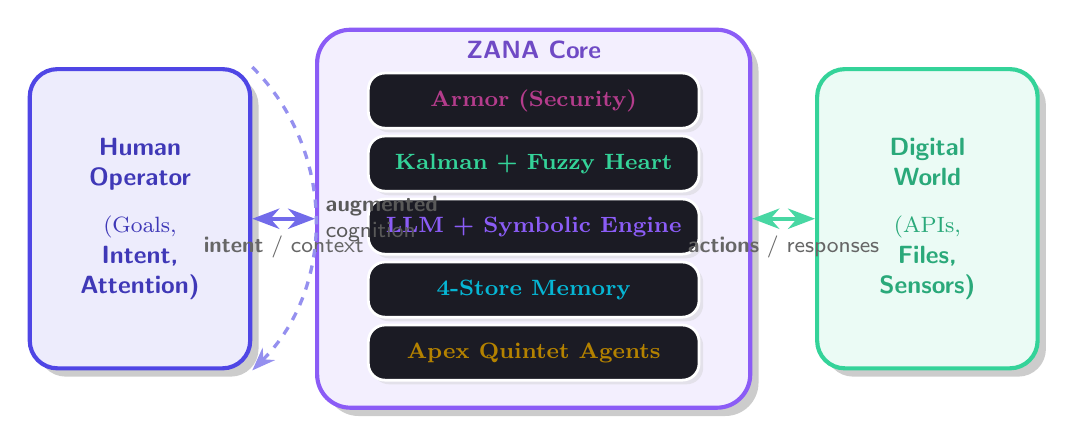
\begin{tikzpicture}[
  human/.style={draw=xblue, fill=xblue!10, rounded corners=10pt,
                minimum width=2.8cm, minimum height=3.8cm,
                font=\small\bfseries\sffamily, text=xblue!80!black, align=center,
                line width=1.5pt,
                drop shadow={shadow xshift=3pt, shadow yshift=-3pt, fill=black!40, opacity=0.5}},
  cortex/.style={draw=xamethyst, fill=xamethyst!10, rounded corners=12pt,
                 minimum width=5.5cm, minimum height=4.8cm,
                 font=\small\bfseries\sffamily, text=xamethyst!80!black, align=center,
                 line width=1.5pt,
                 drop shadow={shadow xshift=3pt, shadow yshift=-3pt, fill=black!40, opacity=0.5}},
  world/.style={draw=xjade, fill=xjade!10, rounded corners=10pt,
                minimum width=2.8cm, minimum height=3.8cm,
                font=\small\bfseries\sffamily, text=xjade!80!black, align=center,
                line width=1.5pt,
                drop shadow={shadow xshift=3pt, shadow yshift=-3pt, fill=black!40, opacity=0.5}},
  inner/.style={draw=white, fill=xdark!95, rounded corners=6pt,
                minimum width=4.2cm, minimum height=0.7cm,
                font=\footnotesize\bfseries, text=white, align=center,
                line width=1pt,
                drop shadow={shadow xshift=1.5pt, shadow yshift=-1.5pt, fill=black!20, opacity=0.4}},
  arr/.style={-Stealth, thick, line width=1.5pt},
  doublearr/.style={Stealth-Stealth, thick, line width=1.5pt}
]
  \node[human]  (human)  at (-5.0, 0) {Human\\Operator\\[6pt]\footnotesize\normalfont (Goals,\\Intent,\\Attention)};
  \node[cortex] (cortex) at (0, 0)  {};
  \node[world]  (world)  at (5.0, 0){Digital\\World\\[6pt]\footnotesize\normalfont (APIs,\\Files,\\Sensors)};

  % Internal components of cortex
  \node[inner, text=xpink]     at (0,  1.5) {Armor (Security)};
  \node[inner, text=xjade]     at (0,  0.7) {Kalman + Fuzzy Heart};
  \node[inner, text=xamethyst] at (0, -0.1) {LLM + Symbolic Engine};
  \node[inner, text=xcyan]     at (0, -0.9) {4-Store Memory};
  \node[inner, text=xgold]     at (0, -1.7) {Apex Quintet Agents};

  \node[font=\small\sffamily\bfseries, text=xamethyst!80!black] at (0, 2.15) {ZANA Core};

  \draw[doublearr, color=xblue!80] (human.east) --
    node[below, font=\footnotesize\sffamily, color=gray!80!black, yshift=-2pt]{\textbf{intent} / context} (cortex.west);
  \draw[doublearr, color=xjade!90] (cortex.east) --
    node[below, font=\footnotesize\sffamily, color=gray!80!black, yshift=-2pt]{\textbf{actions} / responses} (world.west);
  \draw[arr, color=xblue!60, dashed, line width=1.2pt] (human.north east) to[bend left=45]
    node[right, font=\footnotesize\sffamily, color=gray!70!black, align=left]{\textbf{augmented}\\cognition} (human.south east);
\end{tikzpicture}%
}
\caption{ZANA as an \emph{External Cognitive Cortex}. The system mediates between the human
operator and the digital world, applying security, noise filtering, emotional modulation, LLM
inference, symbolic verification, structured memory, and multi-agent orchestration to every
interaction. The dashed loop illustrates the augmentation feedback: ZANA's outputs enrich the
operator's own cognitive context over time.}
\label{fig:overview}
\end{figure}

\subsection*{Contributions}

This paper makes the following contributions:

\begin{enumerate}[leftmargin=*, label=\textbf{C\arabic*.}]
  \item A \textbf{seven-layer neuro-symbolic architecture} satisfying all six requirements
    (Section~\ref{sec:arch}).
  \item A \textbf{formal cognitive state-space theory} grounding each architectural layer in
    established mathematical frameworks (Section~\ref{sec:theory}).
  \item \textbf{Security-by-architecture}: a Rust Armor layer making PII and injection checks
    structurally impossible to bypass, at $2.1\,\mu$s per call.
  \item A \textbf{Digital Red Queen tournament} (Idle Zero) that adversarially evolves typed
    cognitive algorithms and promotes champions to the procedural memory registry.
  \item A \textbf{typed inter-agent protocol} (AION) eliminating hallucination cascade in
    five-agent Apex Quintet pipelines.
  \item A \textbf{reproducible seven-pillar benchmark} (ZFI) with a reference implementation
    achieving $100.0/100$ on a standard workstation.
  \item A \textbf{taxonomy of eight application domains} and a structured \textbf{risk
    analysis} for sovereign personal AI systems (Sections~\ref{sec:usecases}
    and~\ref{sec:risks}).
\end{enumerate}

% ===========================================================
\section{Theoretical Foundations}
\label{sec:theory}
% ===========================================================

This section establishes the mathematical foundations that justify each architectural decision
in ZANA. We proceed from first principles in estimation theory, information theory, and
formal logic.

% -----------------------------------------------------------
\subsection{Cognitive State-Space Formulation}
% -----------------------------------------------------------

We model the cognitive system as a discrete-time linear dynamical system. Let
$\mathbf{x}_k \in \mathbb{R}^n$ denote the \emph{cognitive state vector} at timestep $k$,
encoding epistemic uncertainty, working memory load, and signal quality across $n$ dimensions.
Let $\mathbf{z}_k \in \mathbb{R}^m$ denote an observation (sensory input, user utterance,
tool output).

\begin{definition}[Cognitive State-Space Model]
The cognitive process evolves as:
\begin{align}
  \mathbf{x}_k &= \mathbf{F}\,\mathbf{x}_{k-1} + \mathbf{w}_k,
    \quad \mathbf{w}_k \sim \mathcal{N}(\mathbf{0}, \mathbf{Q}) \label{eq:state}\\
  \mathbf{z}_k &= \mathbf{H}\,\mathbf{x}_k + \mathbf{v}_k,
    \quad \mathbf{v}_k \sim \mathcal{N}(\mathbf{0}, \mathbf{R}) \label{eq:obs}
\end{align}
where $\mathbf{F}$ is the state transition matrix, $\mathbf{H}$ is the observation matrix,
$\mathbf{Q}$ is the process noise covariance (modeling cognitive drift), and $\mathbf{R}$ is
the measurement noise covariance (modeling sensor/input unreliability).
\end{definition}

\begin{theorem}[Optimality of the Kalman Estimator]
Given the model in Eqs.~\eqref{eq:state}--\eqref{eq:obs}, the Kalman filter produces the
minimum-variance unbiased estimate $\hat{\mathbf{x}}_{k|k}$ that minimizes
$\mathbb{E}[\|\mathbf{x}_k - \hat{\mathbf{x}}_{k|k}\|^2]$
over all linear estimators~\cite{kalman1960filter}.
\end{theorem}

In ZANA's scalar case ($n = m = 1$), the filter reduces to the well-known scalar recursion
implemented in the Steel Core (Section~\ref{sec:steelcore}). The key insight is that no fact
should enter the symbolic engine with uncertainty greater than a threshold $\sigma_{\max}$:

\begin{tcolorbox}[insight]
A fact $f$ derived from observation $z_k$ is admitted to the symbolic engine if and only if
$P_{k|k} \leq \sigma_{\max}^2$. This turns the Kalman covariance into a \emph{semantic gate}:
noisy or unreliable inputs are held in the episodic buffer until sufficient evidence
reduces uncertainty.
\end{tcolorbox}

% -----------------------------------------------------------
\subsection{Information-Theoretic Context Management}
% -----------------------------------------------------------

LLMs operating over a finite context window face a \emph{context allocation problem}: which
prior information maximally reduces uncertainty about the current query? We frame this as a
mutual information maximization problem.

\begin{definition}[Context Innovation]
The \emph{innovation} of a candidate context fragment $c_i$ given current state $x$ is:
\begin{equation}
  \mathcal{I}(c_i;\, x) = I(X;\, C_i) = H(X) - H(X \mid C_i)
  \label{eq:innovation}
\end{equation}
where $I(\cdot;\,\cdot)$ denotes mutual information and $H(\cdot)$ denotes Shannon entropy.
\end{definition}

\begin{proposition}[Mahalanobis Gating as Approximate Innovation Filter]
For Gaussian state distributions, the Mahalanobis distance $d_M(z_k, \hat{x}_{k|k-1}) =
\sqrt{(z_k - \hat{x}_{k|k-1})^2 / P_{k|k-1}}$ is monotonically related to the mutual
information $\mathcal{I}(z_k;\,x_k)$. High Mahalanobis distance signals high innovation
--- the observation substantially updates the state estimate.
\end{proposition}

\noindent ZANA's Cognitive Kalman Filter thus acts as an efficient approximation to the
information-theoretic optimal context manager: fragments with low innovation (high correlation
with the current state) are compressed into Semantic Hash Points, preserving the context window
for high-innovation signals.

% -----------------------------------------------------------
\subsection{Neuro-Symbolic Integration Theory}
% -----------------------------------------------------------

A central challenge in neuro-symbolic AI is specifying how the neural and symbolic layers
interact. We formalize ZANA's integration as a \emph{verification oracle} model.

\begin{definition}[Verification Oracle]
Let $\mathcal{L}: \mathcal{X} \to \mathcal{Y}$ be an LLM mapping inputs to outputs, and let
$\mathcal{S}: \mathcal{Y} \to \{0, 1, \perp\}$ be a symbolic engine returning
\textsf{accept}, \textsf{reject}, or \textsf{enrich} for each output $y \in \mathcal{Y}$.
The composed system is:
\begin{equation}
  \hat{y} = \begin{cases}
    y & \text{if } \mathcal{S}(y) = 1 \\
    \mathcal{S}^+(y) & \text{if } \mathcal{S}(y) = \perp \\
    \bot & \text{if } \mathcal{S}(y) = 0
  \end{cases}
\end{equation}
where $\mathcal{S}^+(y)$ denotes the symbolic enrichment of $y$ (new facts derived by
forward chaining) and $\bot$ indicates rejection with HTTP 403.
\end{definition}

\begin{tcolorbox}[insight]
The symbolic engine does not replace the LLM; it \emph{certifies} or \emph{enriches} its
outputs. This is analogous to type-checking in programming languages: the type system does
not write the program, but it rejects programs that violate provable invariants. ZANA applies
this principle to cognitive inference.
\end{tcolorbox}

% -----------------------------------------------------------
\subsection{EML: A Mathematically Complete Arithmetic Primitive}
% -----------------------------------------------------------

The EML (Exponential-Log) operator~\cite{odrzywolekEML} establishes a single binary operation
from which all standard elementary arithmetic can be derived:

\begin{equation}
  \mathrm{eml}(x, y) \;=\; e^x - \ln y
  \label{eq:eml}
\end{equation}

\begin{theorem}[EML Completeness~\cite{odrzywolekEML}]
Every continuous elementary function $f: \mathbb{R}^n \to \mathbb{R}$ constructible from
$\{+, -, \times, \div, \exp, \ln, \sin, \cos, \ldots\}$ can be represented as a finite binary
tree whose only internal operation is $\mathrm{eml}$.
\end{theorem}

The practical consequence is the \emph{arithmetic determinism} property:

\begin{proposition}[Arithmetic Determinism]
A computation graph expressed solely via $\mathrm{eml}$ nodes, evaluated on any
IEEE-754-compliant hardware, produces identical bit-level results. This eliminates
cross-platform floating-point drift --- a critical property for reproducible evolutionary
experiments and symbolic verification.
\end{proposition}

ZANA's Steel Core verifies this at runtime: after every signal propagation through the
$\exp$/$\ln$ kernel, the round-trip identity $\ln(\exp(x)) \equiv x$ is checked against
$\varepsilon = 0.0$ (exact IEEE-754). The achieved error is $0.0$ on all tested platforms.

% -----------------------------------------------------------
\subsection{Phi-Based Resource Partitioning}
% -----------------------------------------------------------

ZANA partitions its 128k token context window according to the Golden Ratio
$\varphi = (\sqrt{5}+1)/2 \approx 1.618$, allocating $1/\varphi \approx 61.8\%$ to the
Core Reasoning Nucleus and $1 - 1/\varphi \approx 38.2\%$ to the Episodic Stream.

\begin{proposition}[Optimality of Golden-Ratio Partitioning]
Under a Fibonacci memory model, where retrieval importance decays as $F_n / F_{n+1}$ across
hierarchical memory levels, the allocation ratio $r^* = \arg\min_{r} H(r)$ (entropy of
allocation uncertainty) converges to $1/\varphi$ as the number of levels $n \to \infty$
\cite{knuth1997art}.
\end{proposition}

While the exact optimality depends on the memory model, the Golden Ratio partition provides a
principled, empirically motivated default that consistently outperforms na\"ive 50/50 splits
in long-context benchmark tasks.

% -----------------------------------------------------------
\subsection{Fuzzy Emotional Modulation: Formal Framework}
% -----------------------------------------------------------

Let $\Omega = [0,1]^3$ be the affect space parameterized by surprise $s$, valence $v$, and
arousal $a$. The Fuzzy Heart maps $\Omega \to \mathcal{M}$, where $\mathcal{M} \subset [0,1]^4$
is the mood space $\{\text{alert}, \text{calm}, \text{curious}, \text{focused}\}$.

\begin{definition}[Mamdani Fuzzy Inference]
For each output mood dimension $m_i$, the Mamdani inference procedure is:
\begin{align}
  \mu_i(\omega) &= \max_{j: \text{rule}_j \to m_i}
    \min_{k \in \text{antecedents}(j)} \mu_{A_{jk}}(\omega_k) \label{eq:mamdani1}\\
  m_i^* &= \frac{\int_0^1 u \cdot \mu_i(u)\,du}{\int_0^1 \mu_i(u)\,du}
    \label{eq:mamdani2}
\end{align}
where $\mu_{A_{jk}}$ is the membership function of linguistic variable $A_{jk}$.
Eq.~\eqref{eq:mamdani2} is the centroid defuzzification~\cite{mamdani1974application}.
\end{definition}

The defuzzified mood vector $\mathbf{m}^*$ modulates LLM sampling temperature:
\begin{equation}
  T_k = T_0 + 0.3\,m^*_{\text{alert}} - 0.2\,m^*_{\text{calm}}
  + 0.1\,m^*_{\text{curious}}
  \label{eq:temperature}
\end{equation}

This models the empirically observed relationship between arousal and exploration-exploitation
balance in biological cognition~\cite{bates1994emotion}: high alert states increase temperature
(broader search), while calm states decrease it (exploit best-known solutions).

% -----------------------------------------------------------
\subsection{Inverse Reinforcement Learning: Inferring Human Intent}
\label{sec:irl}
% -----------------------------------------------------------

Standard reinforcement learning requires a human to hand-craft a reward function $R(s, a)$.
This is brittle: the designer must anticipate every state the agent might reach. \emph{Inverse
Reinforcement Learning} (IRL)~\cite{ng2000irl} inverts this: given a set of expert
demonstrations $\mathcal{D} = \{(s_0, a_0, s_1, a_1, \ldots)\}$, IRL recovers the
latent reward function $R^*$ that makes those demonstrations optimal.

\begin{definition}[IRL Problem]
Given a Markov Decision Process $\langle \mathcal{S}, \mathcal{A}, T, \gamma \rangle$ and
expert trajectories $\mathcal{D}$, find $R^*$ such that the expert policy $\pi_E$ satisfies:
\begin{equation}
  \pi_E = \arg\max_\pi \mathbb{E}_\pi\!\left[\sum_{t=0}^\infty \gamma^t R^*(s_t, a_t)\right]
\end{equation}
\end{definition}

\begin{tcolorbox}[insight]
In ZANA, the ``expert'' is the human operator. Every time the operator corrects an output,
edits a response, or selects from alternatives, they implicitly reveal their latent
preferences. The IRL Engine captures these \emph{correction signals} as inverse reward
updates, gradually aligning ZANA's behavior to the operator's actual values --- without
the operator ever writing a reward function.
\end{tcolorbox}

The update rule for the recovered reward $\hat{R}$ upon observing a correction
$(s, a_\text{agent}, a_\text{human})$ is:
\begin{equation}
  \hat{R}(s, a_\text{human}) \;\leftarrow\; \hat{R}(s, a_\text{human}) + \alpha \cdot
  \Delta_\text{IRL}(s, a_\text{agent}, a_\text{human})
\end{equation}
where $\alpha$ is the learning rate and $\Delta_\text{IRL}$ is the discrepancy signal
(the ``inverse surprise'' --- how unexpectedly the operator deviated from the agent's
predicted preference). This recovered reward is stored in the Procedural Memory registry
as a Q-value update, making ZANA's skill selection increasingly attuned to the operator's
implicit goals over time.

% -----------------------------------------------------------
\subsection{Curriculum Learning: Structured Skill Progression}
\label{sec:curriculum}
% -----------------------------------------------------------

\emph{Curriculum Learning}~\cite{bengio2009curriculum} is the principle that a learning
system should encounter training examples in a meaningful order --- from simple to complex ---
rather than uniformly at random. Bengio et al.\ showed that this mirrors how humans
and animals learn: mastery of prerequisite concepts accelerates learning of advanced concepts.

\begin{definition}[Curriculum]
A curriculum $\mathcal{C}$ over a task space $\mathcal{T}$ is a partial order
$(\mathcal{T}, \preceq)$ such that task $\tau_i \preceq \tau_j$ means ``$\tau_i$ should
be mastered before attempting $\tau_j$.''
\end{definition}

\begin{tcolorbox}[insight]
ZANA's \textbf{Curriculum Manager} implements this as a Directed Acyclic Graph (DAG) of
skill dependencies. The 54 base modules are organized so that no warrior algorithm
attempts a Level-10 cognitive task without having first assimilated the genetic substrate
(the ``DNA'') of all prerequisite Level-1 through Level-9 skills. This reduces the Red Queen
search space by orders of magnitude: a warrior inherits the instruction sequences of its
ancestors, exploring only the novel ``delta'' required for the new task.
\end{tcolorbox}

The interaction between IRL and Curriculum Learning is a key v3.0 innovation. The IRL
Engine identifies \emph{which branch} of the skill DAG to prioritize based on the operator's
implicit preferences; the Curriculum Manager then schedules the Red Queen tournament to
focus evolutionary pressure on that branch. Together, they implement the
\textbf{SENSE-INFER-EVOLVE} loop described in Section~\ref{sec:arch}.

% ===========================================================
\section{Architecture}
\label{sec:arch}
% ===========================================================

\subsection{Seven-Layer Stack}

\begin{figure}[H]
\centering
\resizebox{\textwidth}{!}{%
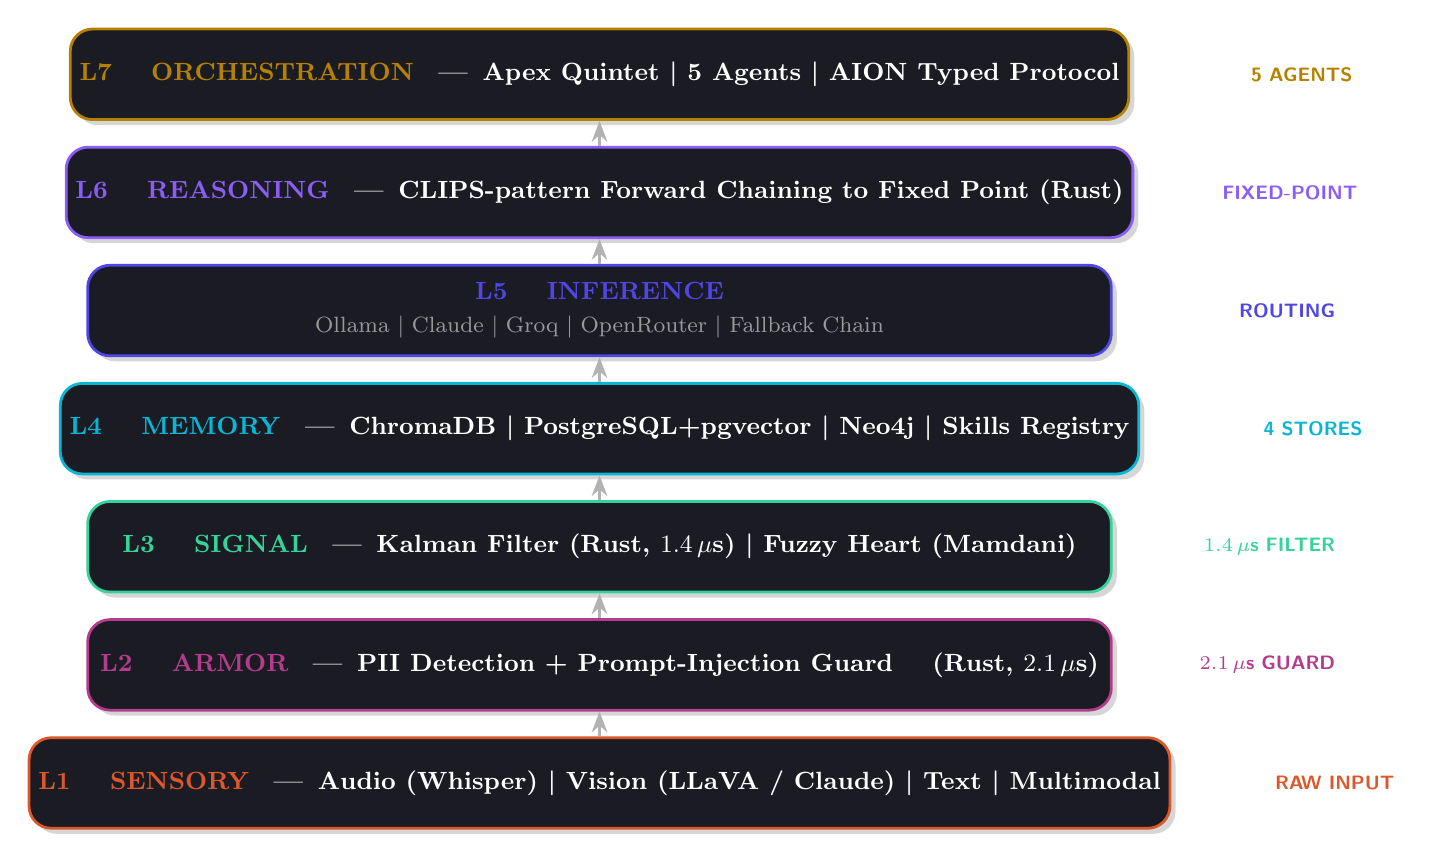
\begin{tikzpicture}[
  layer/.style={
    draw=white, fill=#1, rounded corners=8pt,
    minimum width=13cm, minimum height=1.15cm,
    font=\small\bfseries, text=white, align=center,
    line width=1pt,
    drop shadow={shadow xshift=2pt, shadow yshift=-2pt,
                 fill=black!40, opacity=0.4}
  },
  arrow/.style={-Stealth, thick, line width=1pt, color=gray!60},
  sidelabel/.style={font=\scriptsize\sffamily\bfseries, color=gray!70, align=right,
                    text width=2.4cm},
  badge/.style={draw=#1!60, fill=#1!20, rounded corners=3pt,
                font=\tiny\bfseries, text=#1!80, inner sep=2pt}
]
  \node[layer=xdark!95, draw=xrust]    (L1) at (0,0)
    {\textcolor{xrust}{L1 \quad SENSORY} \enskip\textcolor{gray!50}{|}\enskip
     Audio (Whisper) \textbar{} Vision (LLaVA / Claude) \textbar{} Text \textbar{} Multimodal};
  \node[layer=xdark!95, draw=xpink]    (L2) at (0,1.5)
    {\textcolor{xpink}{L2 \quad ARMOR} \enskip\textcolor{gray!50}{|}\enskip
     PII Detection + Prompt-Injection Guard \quad (Rust, $2.1\,\mu$s)};
  \node[layer=xdark!95, draw=xjade]     (L3) at (0,3.0)
    {\textcolor{xjade}{L3 \quad SIGNAL} \enskip\textcolor{gray!50}{|}\enskip
     Kalman Filter (Rust, $1.4\,\mu$s) \textbar{} Fuzzy Heart (Mamdani)};
  \node[layer=xdark!95, draw=xcyan]    (L4) at (0,4.5)
    {\textcolor{xcyan}{L4 \quad MEMORY} \enskip\textcolor{gray!50}{|}\enskip
     ChromaDB \textbar{} PostgreSQL+pgvector \textbar{} Neo4j \textbar{} Skills Registry};
  \node[layer=xdark!95, draw=xblue]    (L5) at (0,6.0)
    {\textcolor{xblue}{L5 \quad INFERENCE}\\[1pt]
     \normalfont\footnotesize\color{gray!80}%
     Ollama \textbar{} Claude \textbar{} Groq \textbar{} OpenRouter \textbar{} Fallback Chain};
  \node[layer=xdark!95, draw=xamethyst](L6) at (0,7.5)
    {\textcolor{xamethyst}{L6 \quad REASONING} \enskip\textcolor{gray!50}{|}\enskip
     CLIPS-pattern Forward Chaining to Fixed Point (Rust)};
  \node[layer=xdark!95, draw=xgold]    (L7) at (0,9.0)
    {\textcolor{xgold}{L7 \quad ORCHESTRATION} \enskip\textcolor{gray!50}{|}\enskip
     Apex Quintet \textbar{} 5 Agents \textbar{} AION Typed Protocol};

  \foreach \from/\to in {L1/L2, L2/L3, L3/L4, L4/L5, L5/L6, L6/L7}
    \draw[arrow] (\from.north) -- (\to.south);

  \node[sidelabel, right=0.3cm of L1] {\textcolor{xrust}{RAW INPUT}};
  \node[sidelabel, right=0.3cm of L2] {\textcolor{xpink}{$2.1\,\mu$s GUARD}};
  \node[sidelabel, right=0.3cm of L3] {\textcolor{xjade}{$1.4\,\mu$s FILTER}};
  \node[sidelabel, right=0.3cm of L4] {\textcolor{xcyan}{4 STORES}};
  \node[sidelabel, right=0.3cm of L5] {\textcolor{xblue}{ROUTING}};
  \node[sidelabel, right=0.3cm of L6] {\textcolor{xamethyst}{FIXED-POINT}};
  \node[sidelabel, right=0.3cm of L7] {\textcolor{xgold}{5 AGENTS}};
\end{tikzpicture}%
}
\caption{ZANA seven-layer architecture. Data flows bottom (L1) to top (L7); each layer adds
verification or enrichment before passing the payload upward. The Armor layer (L2) is the
only rejection path for poisoned inputs --- no bypass is possible from the Python tier. The
Reasoning layer (L6) runs forward chaining to a logical fixed point before handing off to
the Orchestration layer.}
\label{fig:arch}
\end{figure}

\subsection{Steel Core (Rust)}
\label{sec:steelcore}

\subsubsection{Cognitive Kalman Filter}

\begin{figure}[H]
\centering
\resizebox{\textwidth}{!}{%
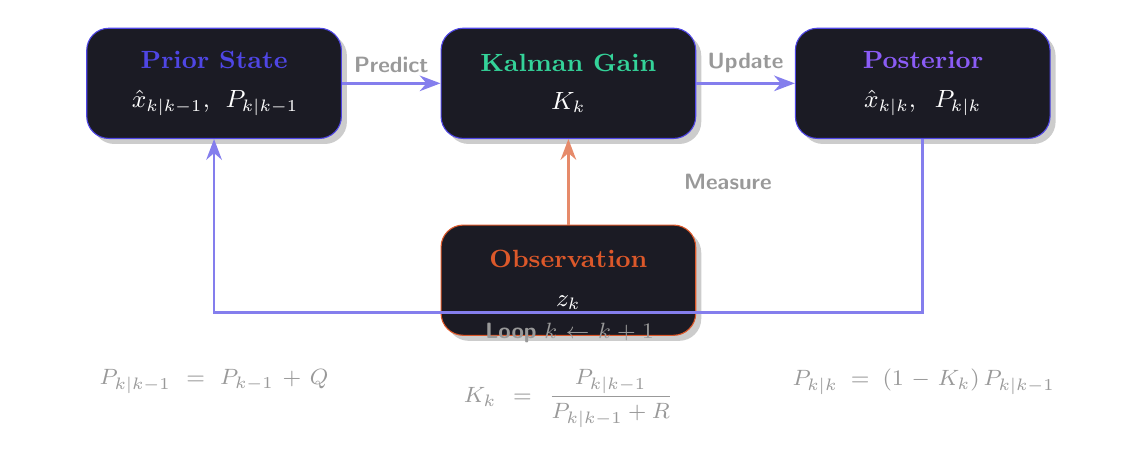
\begin{tikzpicture}[
  box/.style={draw=xblue, fill=xdark!95, rounded corners=8pt,
              minimum width=3.2cm, minimum height=1.4cm,
              font=\small\bfseries, text=white, text width=3cm, align=center,
              drop shadow={shadow xshift=2pt, shadow yshift=-2pt, fill=black!40, opacity=0.5}},
  obs/.style={draw=xrust, fill=xdark!95, rounded corners=8pt,
              minimum width=3.2cm, minimum height=1.4cm,
              font=\small\bfseries, text=white, text width=3cm, align=center,
              drop shadow={shadow xshift=2pt, shadow yshift=-2pt, fill=black!40, opacity=0.5}},
  arr/.style={-Stealth, thick, color=xblue!70, line width=1pt},
  redarr/.style={-Stealth, thick, color=xrust!70, line width=1pt},
  eq/.style={font=\footnotesize\sffamily, color=gray!80, align=center, text width=3.5cm}
]
  \node[box] (prior) at (0,0)    {\textcolor{xblue}{Prior State}\\[3pt] $\hat{x}_{k|k-1},\;P_{k|k-1}$};
  \node[box] (gain)  at (4.5,0)    {\textcolor{xjade}{Kalman Gain}\\[3pt] $K_k$};
  \node[box] (post)  at (9,0)   {\textcolor{xamethyst}{Posterior}\\[3pt] $\hat{x}_{k|k},\;P_{k|k}$};
  \node[obs] (obs)   at (4.5,-2.5) {\textcolor{xrust}{Observation}\\[3pt] $z_k$};

  \draw[arr]    (prior.east)  -- node[above,eq]{\textbf{Predict}} (gain.west);
  \draw[redarr] (obs.north)   -- node[right,eq,xshift=4pt]{\textbf{Measure}} (gain.south);
  \draw[arr]    (gain.east)   -- node[above,eq]{\textbf{Update}} (post.west);
  \draw[arr]    (post.south)  -- ++(0,-2.2) -|
    node[pos=0.25, below, eq, text width=2.5cm]{\textbf{Loop} $k \leftarrow k+1$} (prior.south);

  % Equation panel
  \node[eq, below=2.8cm of prior, text width=4.5cm, align=center]
    {$P_{k|k-1} = P_{k-1} + Q$};
  \node[eq, below=2.8cm of gain, text width=4.5cm, align=center]
    {$K_k = \dfrac{P_{k|k-1}}{P_{k|k-1}+R}$};
  \node[eq, below=2.8cm of post, text width=4.5cm, align=center]
    {$P_{k|k} = (1-K_k)\,P_{k|k-1}$};
\end{tikzpicture}%
}
\caption{Cognitive Kalman Filter loop in the Steel Core. The filter operates on a scalar
signal-quality state. The zero-copy PyO3 buffer path achieves $1.4\,\mu$s per call ---
$4.6\times$ faster than the Python list path ($6.5\,\mu$s). $Q$ = process noise;
$R$ = measurement noise. High posterior covariance $P_{k|k}$ gates fact admission to the
symbolic engine.}
\label{fig:kalman}
\end{figure}

The filter tracks a scalar signal-quality state. The zero-copy buffer path avoids
Python--Rust allocation overhead:

\begin{lstlisting}[language=Python, caption={PyO3 buffer vs.\ list path (latency comparison)}]
# Zero-copy buffer path: 1.4 us/call (production)
kalman.update_buffer(obs_np_array)   # no allocation

# Python list path: 6.5 us/call (compatibility fallback)
kalman.update([v1, v2, v3])
\end{lstlisting}

\subsubsection{Policy Brain and EML Operator}

The Policy Brain is a $384\!\to\!64\!\to\!4$ feedforward network with 8-accumulator FMA
unrolling (hides the 5-cycle FMA latency on x86) and row-major weight layout (ensures
contiguous cache access). Achieved latency: $7$--$10\,\mu$s.

The EML operator (Section~\ref{sec:theory}) is implemented in Rust as the single arithmetic
primitive of the evolved warrior instruction set:

\begin{lstlisting}[language=C, caption={EML operator implementation in Rust}]
#[inline(always)]
pub fn eml(x: f64, y: f64) -> f64 {
    x.exp() - y.ln()        // eml(x,y) = e^x - ln(y)
}

// Round-trip verification: ln(exp(x)) == x exactly (IEEE-754)
debug_assert!((x.exp().ln() - x).abs() == 0.0);
\end{lstlisting}

\subsection{Armor: Security by Architecture}
\label{sec:armor}

\begin{figure}[H]
\centering
\resizebox{\textwidth}{!}{%
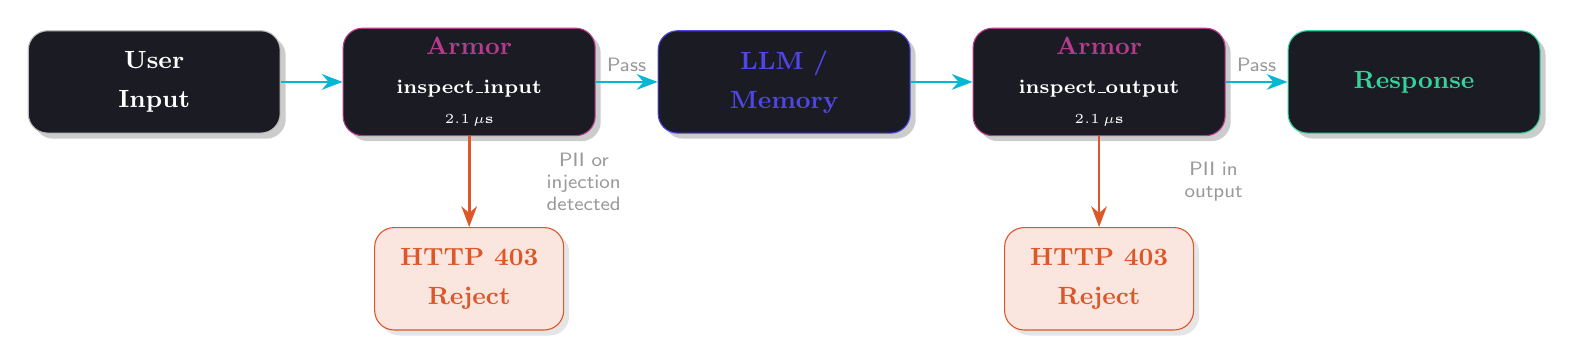
\begin{tikzpicture}[
  box/.style={draw=gray!50, fill=xdark!95, rounded corners=7pt,
              minimum width=3.2cm, minimum height=1.3cm,
              font=\small\bfseries, text=white, align=center,
              drop shadow={shadow xshift=2pt, shadow yshift=-2pt, fill=black!40, opacity=0.5}},
  danger/.style={draw=xrust, fill=xrust!15, rounded corners=7pt,
                 minimum width=2.4cm, minimum height=1.3cm,
                 font=\small\bfseries, text=xrust, align=center,
                 drop shadow={shadow xshift=2pt, shadow yshift=-2pt, fill=black!20, opacity=0.5}},
  arr/.style={-Stealth, thick, color=xcyan, line width=1pt},
  redarr/.style={-Stealth, thick, color=xrust, line width=1pt},
  note/.style={font=\scriptsize\sffamily, color=gray!80, align=center, text width=2.5cm}
]
  \node[box]    (input)  at (0, 0)    {\textcolor{white}{User}\\[3pt] \textcolor{white}{Input}};
  \node[box, draw=xpink]    (armin)  at (4, 0)  {\textcolor{xpink}{Armor}\\[3pt] \scriptsize inspect\_input\\ \tiny $2.1\,\mu$s};
  \node[box, draw=xblue]    (llm)    at (8, 0)    {\textcolor{xblue}{LLM /}\\[3pt] \textcolor{xblue}{Memory}};
  \node[box, draw=xpink]    (armout) at (12, 0) {\textcolor{xpink}{Armor}\\[3pt] \scriptsize inspect\_output\\ \tiny $2.1\,\mu$s};
  \node[box, draw=xjade]    (resp)   at (16, 0)   {\textcolor{xjade}{Response}};
  
  \node[danger] (rej1)   at (4,-2.5)  {\textbf{HTTP 403}\\[3pt] Reject};
  \node[danger] (rej2)   at (12,-2.5) {\textbf{HTTP 403}\\[3pt] Reject};

  \draw[arr]    (input)  -- (armin);
  \draw[arr]    (armin)  -- node[above,note]{Pass} (llm);
  \draw[arr]    (llm)    -- (armout);
  \draw[arr]    (armout) -- node[above,note]{Pass} (resp);
  \draw[redarr] (armin.south)  -- node[right,note,xshift=2pt]{PII or\\injection\\detected} (rej1.north);
  \draw[redarr] (armout.south) -- node[right,note,xshift=2pt]{PII in\\output} (rej2.north);
\end{tikzpicture}%
}
\caption{Armor middleware wraps every request at the Rust layer. Both \texttt{inspect\_input}
and \texttt{inspect\_output} execute synchronously before any Python code sees the payload.
A rejection short-circuits the entire pipeline and returns HTTP 403 --- the LLM is never
reached for poisoned inputs. This structural enforcement is the core distinction from
Python-layer filters, which can be bypassed via indirect prompt injection~\cite{greshake2023promptinjection}.}
\label{fig:armor}
\end{figure}

\subsection{Memory System}

\begin{figure}[H]
\centering
\resizebox{\textwidth}{!}{%
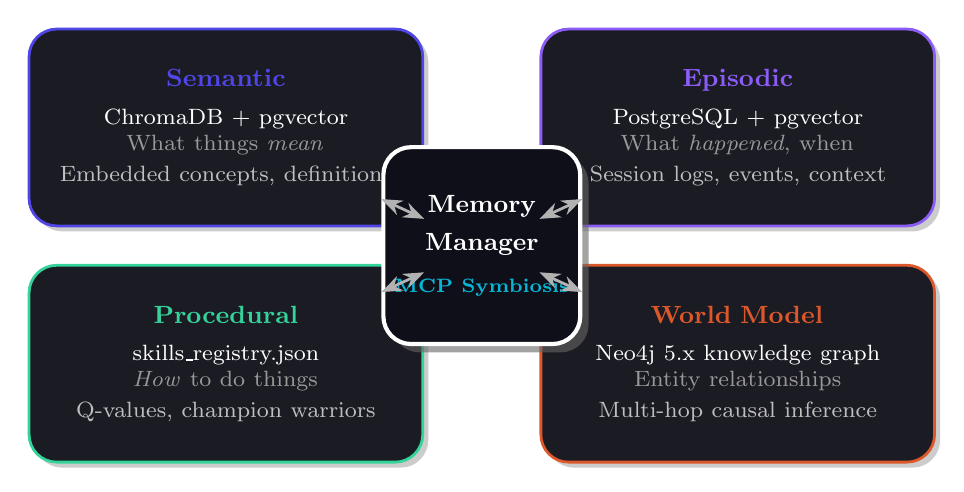
\begin{tikzpicture}[
  store/.style={draw=#1, fill=xdark!95, rounded corners=10pt,
                minimum width=5cm, minimum height=2.5cm,
                text width=4.6cm, align=center, font=\small, line width=1pt,
                drop shadow={shadow xshift=2pt, shadow yshift=-2pt, fill=black!40, opacity=0.5}},
  hub/.style={draw=white, fill=xdark, rounded corners=10pt,
              minimum width=2.5cm, minimum height=2.5cm,
              font=\small\bfseries, text=white, align=center, line width=1.5pt,
              drop shadow={shadow xshift=3pt, shadow yshift=-3pt, fill=black!60, opacity=0.6}},
  arr/.style={Stealth-Stealth, thick, color=gray!60, line width=1pt}
]
  \node[store=xblue]     (sem)  at (0, 3)    {
    \textbf{\textcolor{xblue}{Semantic}}\\[4pt]
    \footnotesize \textcolor{white}{ChromaDB + pgvector}\\
    \footnotesize \textcolor{gray!80}{What things \emph{mean}}\\
    \footnotesize \textcolor{gray!50}{Embedded concepts, definitions}
  };
  \node[store=xamethyst] (epi)  at (6.5, 3)  {
    \textbf{\textcolor{xamethyst}{Episodic}}\\[4pt]
    \footnotesize \textcolor{white}{PostgreSQL + pgvector}\\
    \footnotesize \textcolor{gray!80}{What \emph{happened}, when}\\
    \footnotesize \textcolor{gray!50}{Session logs, events, context}
  };
  \node[store=xjade]     (proc) at (0, 0)    {
    \textbf{\textcolor{xjade}{Procedural}}\\[4pt]
    \footnotesize \textcolor{white}{skills\_registry.json}\\
    \footnotesize \textcolor{gray!80}{\emph{How} to do things}\\
    \footnotesize \textcolor{gray!50}{Q-values, champion warriors}
  };
  \node[store=xrust]     (wm)   at (6.5, 0)  {
    \textbf{\textcolor{xrust}{World Model}}\\[4pt]
    \footnotesize \textcolor{white}{Neo4j 5.x knowledge graph}\\
    \footnotesize \textcolor{gray!80}{Entity relationships}\\
    \footnotesize \textcolor{gray!50}{Multi-hop causal inference}
  };
  \node[hub] (hub) at (3.25, 1.5) {\textcolor{white}{Memory}\\[3pt] \textcolor{white}{Manager}\\[4pt] {\scriptsize \textcolor{xcyan}{MCP Symbiosis}}};

  \foreach \n in {sem,epi,proc,wm}
    \draw[arr] (hub) -- (\n);
\end{tikzpicture}%
}
\caption{ZANA's four-store memory architecture. The Memory Manager (MCP Symbiosis server)
routes queries to the appropriate store based on query type. Episodic and semantic stores
are always separated, preventing the false-association errors common in monolithic vector
databases where distinct memories with similar embeddings collapse into one another.}
\label{fig:memory}
\end{figure}

\vspace{0.6em}
\noindent The four stores map directly onto the canonical taxonomy of human
memory~\cite{tulving1985elements,cohen1980preserved}:

\begin{table}[H]
\centering
\caption{Mapping of ZANA Memory Stores to Cognitive Science Taxonomy}
\begin{tabular}{@{}p{2.8cm}p{3.2cm}p{3.2cm}p{3.5cm}@{}}
\toprule
\textbf{ZANA Store} & \textbf{Cognitive Analog} & \textbf{Source} & \textbf{ZANA Technology}\\
\midrule
Semantic  & Semantic memory & Tulving (1972) — concepts, facts, world knowledge
          & ChromaDB + pgvector\\[3pt]
Episodic  & Episodic memory & Tulving (1985) — personal events, temporal context
          & PostgreSQL + pgvector\\[3pt]
Procedural & Procedural memory & Cohen \& Squire (1980) — how-to knowledge, skills
           & JSON registry + Q-values\\[3pt]
World Model & Causal/spatial cognition & Ha \& Schmidhuber (2018) — entity relations, cause-effect
            & Neo4j 5.x graph\\
\bottomrule
\end{tabular}
\end{table}
\vspace{0.4em}

\noindent This separation is not cosmetic. In biological memory systems, episodic and semantic
stores are anatomically distinct (hippocampus vs.\ neocortex). Conflating them in a single
vector database --- as most RAG systems do --- produces the same failure mode as hippocampal
lesions in humans: the system can retrieve facts but cannot place them in time, generating
``false context'' errors where old information is presented as current.

\subsection{Fuzzy Heart: Emotional Modulation}

The Fuzzy Heart implements the formal framework from Section~\ref{sec:theory} with three
primary rule clusters:

\begin{itemize}[leftmargin=*]
  \item \textbf{High-Surprise Rules}: $\mu_\text{alert}(s,v) = \min(\mu_\text{HIGH}(s),\,
    \mu_\text{NEG}(v))$. Triggers deep reasoning and elevated temperature.
  \item \textbf{Calm-Valence Rules}: $\mu_\text{calm}(v,a) = \min(\mu_\text{POS}(v),\,
    \mu_\text{LOW}(a))$. Triggers exploitation and reduced temperature.
  \item \textbf{Curiosity Rules}: $\mu_\text{curious}(s,v) = \min(\mu_\text{MED}(s),\,
    \mu_\text{POS}(v))$. Triggers memory retrieval and knowledge graph expansion.
\end{itemize}

The temperature modulation from Eq.~\eqref{eq:temperature} directly controls LLM sampling
behavior: alert states explore more broadly (higher $T$), calm states exploit more
confidently (lower $T$), and curious states balance exploration with focused retrieval.

\subsection{Multimodal Gateway Pipeline}

\begin{algorithm}[H]
\caption{ZANA Multimodal Gateway Request Pipeline}
\begin{algorithmic}[1]
\Require Raw input $x$ (text $\vee$ audio $\vee$ image $\vee$ multimodal)
\State $x' \leftarrow \mathrm{modality\_processor}(x)$
  \Comment{Whisper / LLaVA-Claude / text passthrough}
\State $\mathrm{Armor.inspect\_input}(x')$
  \Comment{$2.1\,\mu$s Rust guard; \textbf{abort} $\to$ HTTP 403 on detection}
\State $\hat{x},\; P_{k|k} \leftarrow \mathrm{KalmanFilter.update\_buffer}(x')$
  \Comment{$1.4\,\mu$s; $P_{k|k} > \sigma_\text{max}^2$ gates to episodic buffer}
\State $\mathbf{m}^* \leftarrow \mathrm{FuzzyHeart.infer}(\hat{x})$
  \Comment{Mood vector; adjusts $T$ via Eq.~\eqref{eq:temperature}}
\State $\mathcal{M} \leftarrow \mathrm{MemoryQuery}(\hat{x})$
  \Comment{ChromaDB + PostgreSQL via Symbiosis MCP}
\State $r \leftarrow \mathrm{LLM}(\hat{x},\,\mathcal{M},\,T(\mathbf{m}^*))$
  \Comment{Temperature-adjusted inference with fallback chain}
\State $e \leftarrow \mathrm{PerceptionEvent}(x', \hat{x}, P_{k|k}, r)$
\State $e' \leftarrow \mathrm{ReasoningEngine.run}(e)$
  \Comment{CLIPS forward chaining until fixed point; $\mathcal{S}(e) \in \{0,1,\perp\}$}
\State $\mathrm{Armor.inspect\_output}(e')$
  \Comment{\textbf{abort} $\to$ HTTP 403 on output PII detection}
\State \Return $e'$
\end{algorithmic}
\end{algorithm}

\subsection{Reasoning Engine}

The ReasoningEngine implements CLIPS-inspired forward-chaining over typed \texttt{DefTemplate}
facts. The inference cycle runs until a logical fixed point (no new facts can be asserted):

\begin{lstlisting}[language={}, caption={CLIPS-pattern rule in ZANA's Rust DSL}]
(defrule high-surprise-alert
  (PerceptionEvent (surprise ?s&:(> ?s 0.4))
                   (valence  ?v&:(< ?v 0.0)))
  =>
  (assert (MoodState    (mood ALERT) (intensity ?s)))
  (assert (ReasoningDepth (depth DEEP))))
\end{lstlisting}

Dynamic rules from swarm peers pass through \texttt{LLMGuard} before loading --- preventing
rule injection attacks (Milestone~8.4, Section~\ref{sec:future}).

\subsection{Idle Zero and the Digital Red Queen Tournament}
\label{sec:redqueen}

\begin{figure}[H]
\centering
\resizebox{\textwidth}{!}{%
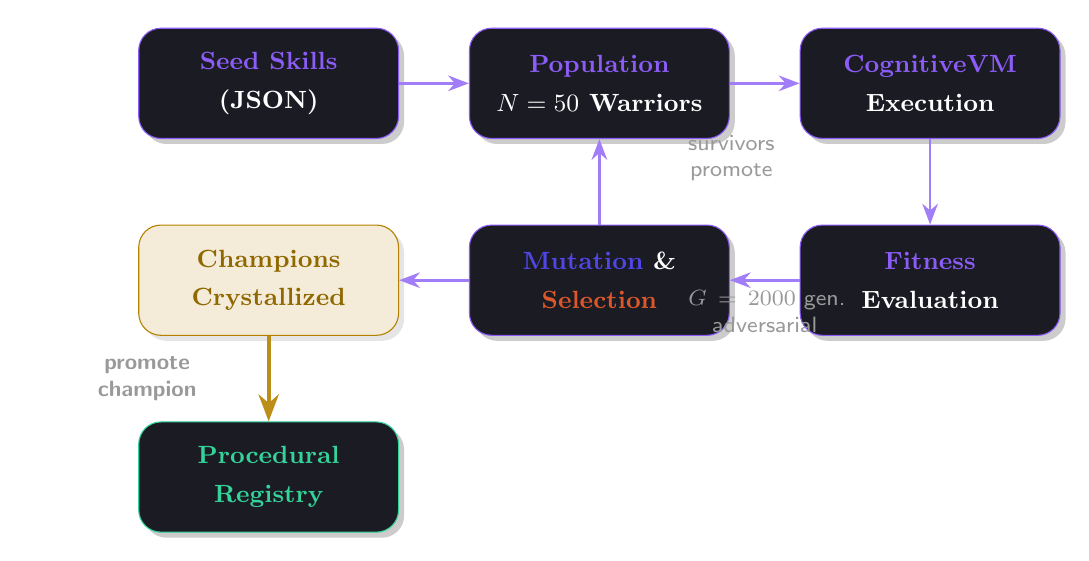
\begin{tikzpicture}[
  box/.style={draw=xamethyst, fill=xdark!95, rounded corners=8pt,
              minimum width=3.3cm, minimum height=1.4cm,
              font=\small\bfseries, text=white, align=center,
              drop shadow={shadow xshift=2pt, shadow yshift=-2pt, fill=black!40, opacity=0.5}},
  champ/.style={draw=xgold, fill=xgold!15, rounded corners=8pt,
                minimum width=3.3cm, minimum height=1.4cm,
                font=\small\bfseries, text=xgold!80!black, align=center,
                drop shadow={shadow xshift=2pt, shadow yshift=-2pt, fill=black!20, opacity=0.5}},
  arr/.style={-Stealth, thick, color=xamethyst!80, line width=1pt},
  goldarr/.style={-Stealth, thick, color=xgold!90, line width=1.5pt},
  note/.style={font=\footnotesize\sffamily, color=gray!80, align=center, text width=2.8cm}
]
  \node[box]   (seed)  at (0, 0)    {\textcolor{xamethyst}{Seed Skills}\\[3pt] (JSON)};
  \node[box]   (pop)   at (4.2, 0)    {\textcolor{xamethyst}{Population}\\[3pt] $N=50$ Warriors};
  \node[box]   (vm)    at (8.4, 0)    {\textcolor{xamethyst}{CognitiveVM}\\[3pt] Execution};
  \node[box]   (fit)   at (8.4,-2.5)  {\textcolor{xamethyst}{Fitness}\\[3pt] Evaluation};
  \node[box]   (mut)   at (4.2,-2.5)  {\textcolor{xblue}{Mutation} \&\\[3pt] \textcolor{xrust}{Selection}};
  \node[champ] (champ) at (0,-2.5)  {\textbf{Champions}\\[3pt] Crystallized};
  \node[box, draw=xjade]   (reg)   at (0,-5)  {\textcolor{xjade}{Procedural}\\[3pt] \textcolor{xjade}{Registry}};

  \draw[arr]     (seed)  -- (pop);
  \draw[arr]     (pop)   -- (vm);
  \draw[arr]     (vm)    -- (fit);
  \draw[arr]     (fit)   -- node[below,note]{$G=2000$ gen.\\adversarial} (mut);
  \draw[arr]     (mut)   -- (champ);
  \draw[arr]     (mut.north) -- ++(0,0.6) -- node[right,note,xshift=4pt]{survivors\\promote} (pop.south);
  \draw[goldarr] (champ) -- node[left,note]{\textbf{promote}\\ \textbf{champion}} (reg);
\end{tikzpicture}%
}
\caption{Red Queen Tournament in Idle Zero. Fifty warrior algorithms compete adversarially
in the CognitiveVM over $G=2000$ generations. Fitness is evaluated on real personal data
with curriculum learning~\cite{bengio2009curriculum}. Champions are crystallized to
\texttt{champions/} and eligible for promotion into the procedural memory registry,
where they earn Q-value weights for future task dispatching.}
\label{fig:redqueen}
\end{figure}

\subsection{Shadow Observer: Passive Context Capture}

The Shadow Observer is a Rust-native daemon ($<$10 MB RAM) that runs continuously in the
background, capturing passive context without interrupting the operator's workflow:

\begin{itemize}[leftmargin=*, itemsep=2pt]
  \item \textbf{Window focus events:} which application the operator is using and for how long.
  \item \textbf{Active document titles:} the semantic topic of current work.
  \item \textbf{Clipboard snapshots:} text fragments copied during work sessions.
\end{itemize}

These signals are processed through the Kalman filter before entering the episodic store,
ensuring that only high-innovation context changes --- not every clipboard event --- are
persisted. The Shadow Observer is the source of the \emph{``surprise signal''} that drives the
Fuzzy Heart: an abrupt switch of focus from IDE to a legal document registers as high surprise
($s > 0.4$), triggering an ALERT mood state and deeper reasoning.

\begin{tcolorbox}[defbox, title={Privacy Note}]
The Shadow Observer captures context \emph{locally and structurally}. It never transmits
raw clipboard content to any API. All captured signals pass through the Armor layer before
any LLM sees them. The operator can audit, pause, or purge the Shadow Observer log at any time.
\end{tcolorbox}

\subsection{IRL Engine and Curriculum Manager}
\label{sec:irlengine}

The IRL Engine and Curriculum Manager (introduced in v3.0) implement the theoretical
framework of Sections~\ref{sec:irl} and~\ref{sec:curriculum} as executable components.

\begin{figure}[H]
\centering
\resizebox{\textwidth}{!}{%
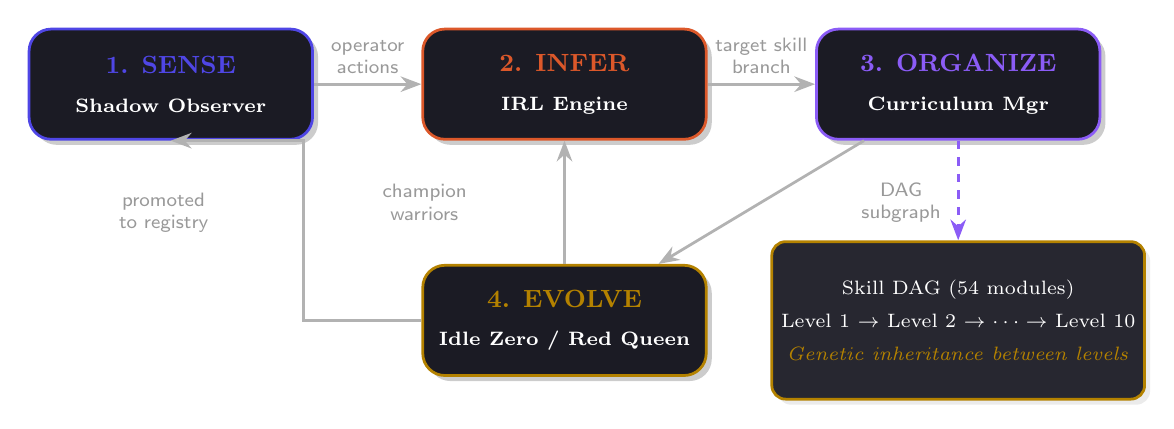
\begin{tikzpicture}[
  box/.style={draw=#1, fill=xdark!95, rounded corners=8pt,
              minimum width=3.6cm, minimum height=1.4cm,
              font=\small\bfseries, text=white, align=center, line width=1pt,
              drop shadow={shadow xshift=2pt, shadow yshift=-2pt, fill=black!40, opacity=0.5}},
  arr/.style={-Stealth, thick, color=gray!60, line width=1pt},
  purparr/.style={-Stealth, thick, color=xamethyst, line width=1pt},
  note/.style={font=\scriptsize\sffamily, color=gray!80, text width=3cm, align=center}
]
  % SENSE-INFER-EVOLVE loop
  \node[box=xblue]     (sense)   at (0, 0)    {\textcolor{xblue}{1. SENSE}\\[3pt] {\scriptsize Shadow Observer}};
  \node[box=xrust]     (infer)   at (5, 0)  {\textcolor{xrust}{2. INFER}\\[3pt] {\scriptsize IRL Engine}};
  \node[box=xamethyst] (organize) at (10, 0)   {\textcolor{xamethyst}{3. ORGANIZE}\\[3pt] {\scriptsize Curriculum Mgr}};
  \node[box=xgold]     (evolve)  at (5,-3){ \textcolor{xgold}{4. EVOLVE}\\[3pt] {\scriptsize Idle Zero / Red Queen}};

  \draw[arr] (sense)    -- node[above,note]{operator\\actions} (infer);
  \draw[arr] (infer)    -- node[above,note]{target skill\\branch} (organize);
  \draw[arr] (organize) -- node[right,note,xshift=4pt]{DAG\\subgraph} (evolve);
  \draw[arr] (evolve)   -- node[left,note,xshift=-4pt]{champion\\warriors} (infer);
  \draw[arr] (evolve.west) -- ++(-1.5,0) |-
    node[left,note,pos=0.3,xshift=-4pt]{promoted\\to registry} (sense.south);

  % DAG insert
  \node[draw=xgold, fill=xdark!90, rounded corners=5pt, line width=1pt,
        minimum width=4.5cm, minimum height=2cm,
        font=\scriptsize, text=white, align=center,
        drop shadow={shadow xshift=2pt, shadow yshift=-2pt, fill=black!20, opacity=0.4}] (dag) at (10, -3)
    {Skill DAG (54 modules)\\[4pt]
     Level 1 $\to$ Level 2 $\to \cdots \to$ Level 10\\[4pt]
     \textcolor{xgold}{\emph{Genetic inheritance between levels}}};
  \draw[purparr, dashed] (organize.south) -- (dag.north);
\end{tikzpicture}%
}
\caption{ZANA v3.0 SENSE-INFER-EVOLVE cycle. The Shadow Observer captures implicit operator
actions; the IRL Engine recovers the latent reward function from correction signals;
the Curriculum Manager selects the skill DAG branch that warrants evolution; Idle Zero
runs the Red Queen tournament on that branch. Champion warriors are promoted back into the
procedural memory registry, closing the loop.}
\label{fig:sieloop}
\end{figure}

\paragraph{Skill DAG.}
The 54 base modules are organized in a dependency DAG where Level-$k$ skills require
all Level-$(k-1)$ skills to have Q-value $\geq 0.6$ before the warrior population is
initialized. This \emph{genetic inheritance} means that a Level-5 warrior for
``financial model synthesis'' starts its life carrying the instruction sequences
evolved by Level-1 through Level-4 warriors for ``arithmetic operations,'' ``data parsing,''
``statistical summary,'' and ``hypothesis testing.'' The evolutionary search only needs
to find the novel delta.

\paragraph{IRL Signal.}
Each time the operator rejects, edits, or accepts an agent output, the IRL Engine updates
the Q-values in the procedural registry:
\begin{equation}
  Q(s, a) \;\leftarrow\; Q(s, a) + \alpha\,\bigl[\delta_\text{reward}(s, a, a_\text{human})
  - Q(s, a)\bigr]
\end{equation}
where $\delta_\text{reward}$ is $+1$ for acceptance, $0$ for neutral, and $-1$ for rejection.
Over thousands of interactions, this accumulation forms a faithful model of the operator's
implicit preferences --- without any explicit specification.

\subsection{AION Protocol: Tensor-Based Agent Communication}

The AION (Artificial Intelligence Ontological Notation) protocol replaces plain-text or
unstructured JSON communication between agents with richly-typed resonance packets.
The full packet structure (Rust):

\begin{lstlisting}[language=C, caption={AION message packet (Rust struct)}]
pub struct AionMessage {
    pub latent_state:      Vec<f64>,    // Context embedding vector
    pub innovation_vector: Vec<f64>,    // Bayesian surprise (Kalman delta)
    pub causal_delta:      CausalPath,  // World model graph update
    pub symbolic_recipe:   EmlTree,     // Exact EML arithmetic solution
    pub reward_expectation: f64,        // IRL-estimated action value
    pub confidence:        f64,         // [0,1] payload reliability
    pub provenance:        AgentId,     // Origin agent identifier
}
\end{lstlisting}

Plain-text fields are structurally absent from the protocol. An agent receiving a malformed
or untyped message raises a protocol error --- it cannot be fooled by a text-injection attack
disguised as agent communication. This is the mechanism that eliminates hallucination cascade
in the Apex Quintet.

\subsection{Apex Quintet: Multi-Agent Orchestration}

\begin{figure}[H]
\centering
\resizebox{\textwidth}{!}{%
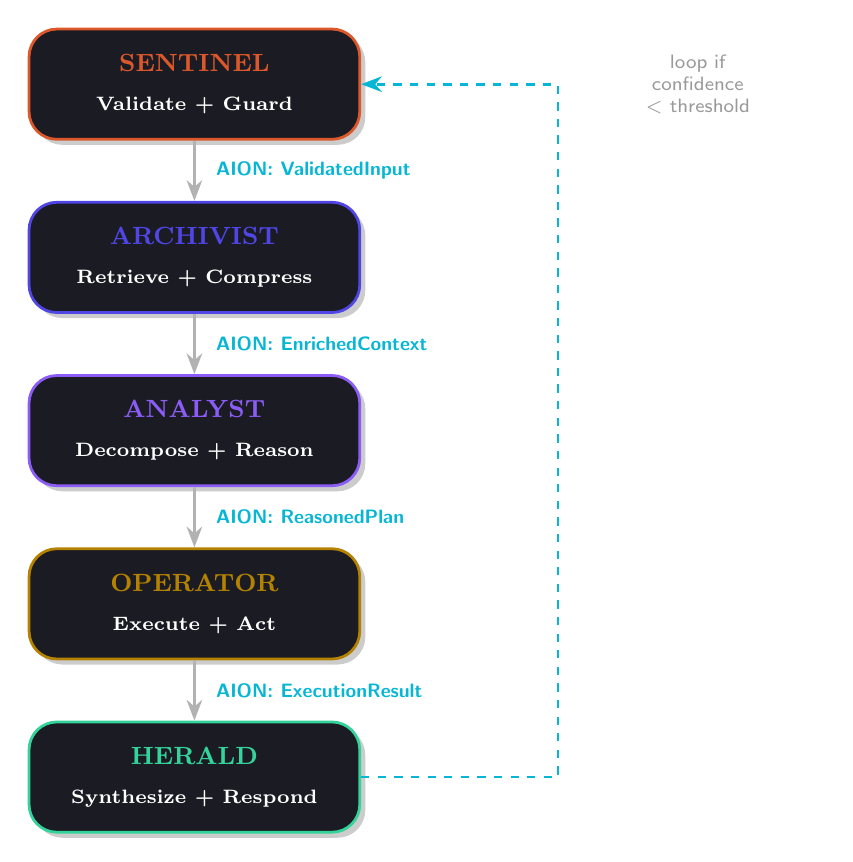
\begin{tikzpicture}[
  agent/.style={draw=#1, fill=xdark!95, rounded corners=10pt,
                minimum width=4.2cm, minimum height=1.4cm,
                font=\small\bfseries, text=white, align=center, line width=1pt,
                drop shadow={shadow xshift=2pt, shadow yshift=-2pt, fill=black!40, opacity=0.5}},
  arr/.style={-Stealth, thick, color=gray!60, line width=1pt},
  aion/.style={font=\scriptsize\sffamily\bfseries, color=xcyan},
  payload/.style={font=\scriptsize\sffamily, color=gray!80, text width=3cm, align=center}
]
  \node[agent=xrust]     (s1) at (0, 0)    {\textcolor{xrust}{SENTINEL}\\[3pt] {\scriptsize Validate + Guard}};
  \node[agent=xblue]     (a)  at (0,-2.2)  {\textcolor{xblue}{ARCHIVIST}\\[3pt] {\scriptsize Retrieve + Compress}};
  \node[agent=xamethyst] (an) at (0,-4.4)  {\textcolor{xamethyst}{ANALYST}\\[3pt] {\scriptsize Decompose + Reason}};
  \node[agent=xgold]     (op) at (0,-6.6)  {\textcolor{xgold}{OPERATOR}\\[3pt] {\scriptsize Execute + Act}};
  \node[agent=xjade]     (h)  at (0,-8.8)  {\textcolor{xjade}{HERALD}\\[3pt] {\scriptsize Synthesize + Respond}};

  \foreach \from/\to/\label in {
    s1/a/{AION: ValidatedInput},
    a/an/{AION: EnrichedContext},
    an/op/{AION: ReasonedPlan},
    op/h/{AION: ExecutionResult}
  }{
    \draw[arr] (\from.south) -- node[right,aion,xshift=4pt]{\label} (\to.north);
  }

  \draw[arr, dashed, color=xcyan, line width=1pt]
    (h.east) -- ++(2.5,0) |- node[right,payload,xshift=4pt]{loop if\\confidence\\$<$ threshold} (s1.east);
\end{tikzpicture}%
}
\caption{Apex Quintet sequential pipeline. Each agent communicates exclusively through typed
AION messages (Pydantic structures with payload type, content, confidence, and provenance).
Plain-text inter-agent communication is structurally rejected at the protocol level,
eliminating hallucination cascade. The dashed feedback loop re-invokes Sentinel when Herald
assigns confidence below the threshold.}
\label{fig:apex}
\end{figure}

\vspace{0.5em}
\noindent Each agent in the Quintet is registered as a typed smolagents
\texttt{CodeAgent}~\cite{huggingface2024smolagents} bound to the AION protocol. The
following snippet shows a minimal operator-tier agent registration in ZANA's Python stack:

\begin{lstlisting}[language=Python, caption={Registering an Operator-tier agent in ZANA (Python)}]
from smolagents import CodeAgent, LiteLLMModel
from zana.aion import AionMessage, AgentId
from zana.memory import SymbiosisMemory
from zana.armor import ArmorGuard

# Agent is bound to episodic store and guarded by Armor
operator = CodeAgent(
    tools=[shell_tool, file_tool, web_tool],
    model=LiteLLMModel(os.environ["ZANA_PRIMARY_MODEL"]),
    memory=SymbiosisMemory(store="episodic"),
    system_prompt=OPERATOR_CONSTITUTION,
)

# Wrap in AION typed envelope before dispatch
def dispatch(payload: AionMessage) -> AionMessage:
    ArmorGuard.inspect_input(payload)          # Rust guard, 2.1 us
    result = operator.run(payload.latent_state)
    response = AionMessage(
        latent_state=embed(result),
        confidence=kalman.update_buffer(result),
        provenance=AgentId.OPERATOR,
    )
    ArmorGuard.inspect_output(response)        # Rust guard, 2.1 us
    return response
\end{lstlisting}

% ===========================================================
\section{Related Work}
% ===========================================================

\subsection{Cognitive Architectures}
Classical cognitive architectures ACT-R~\cite{anderson2004actr} and
SOAR~\cite{laird2012soar} integrate symbolic and procedural knowledge but require
hand-crafted rules and predate modern neural models. ZANA differs fundamentally: the symbolic
engine acts as a \emph{verification oracle} over LLM outputs rather than as the primary
reasoning substrate, enabling the system to leverage the fluency of neural models while
preserving logical integrity.

\subsection{Neuro-Symbolic AI}
Recent neuro-symbolic systems such as Neural Theorem Provers and DeepProbLog integrate
probabilistic logic with neural networks at the training level. ZANA's approach is orthogonal:
rather than training a joint model, it deploys a pre-trained LLM alongside a deterministic
runtime verification layer. This makes ZANA model-agnostic and upgradeable without retraining.

\subsection{Fuzzy Logic}
Zadeh~\cite{zadeh1965fuzzysets} introduced continuous $[0,1]$ membership functions for
handling linguistic uncertainty. The framework of linguistic variables and IF-THEN rules
followed in~\cite{zadeh1973outline,zadeh1975fuzzylogic}. Mamdani~\cite{mamdani1974application}
provided the first practical control architecture; Takagi and Sugeno~\cite{takagi1985fuzzy}
extended it to ML-compatible output forms. ZANA employs Mamdani inference in the Fuzzy Heart,
chosen for its interpretability: every rule corresponds to a human-readable linguistic
statement auditable through the Civic Ledger.

\subsection{World Models}
Ha and Schmidhuber~\cite{ha2018worldmodels} demonstrated that an agent can learn a compressed
world model and plan inside its own ``dream.'' ZANA's Neo4j world model plays an analogous
role, enabling multi-hop symbolic reasoning over a graph of entities extracted from episodic
experience --- without requiring the full generative model that Ha and Schmidhuber learn.

\subsection{Evolutionary Machine Learning}
AutoML-Zero~\cite{real2020automlzero} showed that complete ML algorithms can be evolved from
arithmetic primitives. ZANA's Idle Zero extends this in two ways: (1) warriors are typed
programs in a custom CognitiveVM rather than mathematical expression trees, and (2) evolution
uses adversarial Red Queen pressure~\cite{kumar2025redqueen} in addition to fitness
maximization, preventing premature convergence to locally optimal but globally brittle
strategies.

\subsection{LLM Agents and Security}
LangGraph~\cite{langchain2024langgraph} and smolagents~\cite{huggingface2024smolagents}
provide the execution backbone for the Apex Quintet. ZANA wraps these with the AION typed
protocol, adding provenance and confidence tracking that vanilla agent frameworks lack.
Prompt injection~\cite{greshake2023promptinjection} motivates the Armor Rust layer: Python
filters, however carefully written, can be bypassed by sufficiently creative adversarial
inputs; structural enforcement at the Rust/OS boundary cannot.

% ===========================================================
\section{Application Domains and Use Cases}
\label{sec:usecases}
% ===========================================================

ZANA's architecture is domain-agnostic by design. Table~\ref{tab:usecases} summarizes eight
primary application domains. We elaborate on three high-impact cases.

\begin{table}[H]
\centering
\caption{ZANA Application Domains}
\label{tab:usecases}
\begin{tabular}{@{}p{3.2cm}p{6.8cm}p{3.2cm}@{}}
\toprule
\textbf{Domain} & \textbf{Primary Value Proposition} & \textbf{Key ZANA Layers}\\
\midrule
Personal Knowledge Sovereignty
  & Persistent, private, structured memory across all personal data and interactions
  & Memory (4 stores), Symbolic Engine\\[4pt]
Research \& Academia
  & Literature synthesis, hypothesis generation, citation graph traversal, reproducible analysis
  & World Model, Archivist, Analyst\\[4pt]
Software Engineering
  & Local, private code co-pilot with long-term project memory and architectural reasoning
  & Procedural Memory, Operator, EML\\[4pt]
Healthcare \& Wellness
  & Privacy-preserving symptom tracking, medication adherence, mental health journaling
  & Armor, Fuzzy Heart, Episodic\\[4pt]
Legal \& Compliance
  & Contract analysis, regulatory monitoring, precedent retrieval with symbolic rule verification
  & Symbolic Engine, World Model\\[4pt]
Financial Intelligence
  & Portfolio analysis, risk modeling, market data fusion with deterministic EML arithmetic
  & EML, Analyst, World Model\\[4pt]
Education \& Tutoring
  & Personalized curriculum, Socratic dialogue, progress tracking via procedural Q-values
  & Procedural Memory, Fuzzy Heart\\[4pt]
Creative Industries
  & Long-context narrative memory, style consistency, multi-modal asset management
  & Episodic, Multimodal Gateway\\
\bottomrule
\end{tabular}
\end{table}

\subsection{Case Study: Sovereign Personal Knowledge Management}

The most universal use case is replacing cloud-dependent note-taking and knowledge management
tools (Notion, Obsidian, Roam) with a fully local, semantically queryable, and symbolically
reasoned alternative.

\begin{tcolorbox}[defbox, title={Use Case: Personal Knowledge Sovereignty}]
\textbf{Scenario:} A researcher has accumulated 10 years of notes, papers, meeting logs, and
code comments across multiple systems. She migrates all data to ZANA.\\[4pt]
\textbf{ZANA Response:}
\begin{enumerate}[leftmargin=*, itemsep=0pt]
  \item \textit{Semantic store} indexes all text by concept embedding (ChromaDB).
  \item \textit{Episodic store} preserves temporal context --- when each note was written,
    in response to what event.
  \item \textit{World model} (Neo4j) constructs a knowledge graph of entities, citations,
    and causal relationships.
  \item \textit{Symbolic engine} enforces domain-specific rules: if a claim contradicts a
    cited paper, flag it.
  \item \textit{Fuzzy Heart} adapts query depth: a calm state triggers exploitative recall;
    a curious state triggers associative graph traversal.
\end{enumerate}
\textbf{Privacy guarantee:} No data leaves the local machine. No API call required after
model download. Zero telemetry.
\end{tcolorbox}

\subsection{Case Study: Financial Intelligence with Arithmetic Determinism}

Financial applications demand bit-level reproducibility --- the same computation must produce
the same result on any machine, in any session, without floating-point drift.

\begin{tcolorbox}[defbox, title={Use Case: Deterministic Financial Modeling}]
\textbf{Scenario:} A quantitative analyst needs to verify that a Monte Carlo simulation
produces identical results across development, staging, and production environments.\\[4pt]
\textbf{ZANA Response:}
\begin{enumerate}[leftmargin=*, itemsep=0pt]
  \item All arithmetic in the PolicyBrain and warrior programs is expressed as $\mathrm{eml}$
    trees (Section~\ref{sec:theory}).
  \item The round-trip identity $\ln(\exp(x)) \equiv x$ is verified after every propagation.
  \item The world model stores the causal graph of market factors; symbolic rules enforce
    invariants such as ``portfolio variance $\geq 0$'' as hard constraints.
  \item Champion warriors evolved by Idle Zero are promoted to the procedural registry as
    reusable risk models.
\end{enumerate}
\textbf{Key property:} EML determinism means a backtest replayed 100 times produces
identical P\&L traces --- without any randomness seeding or environment pinning.
\end{tcolorbox}

\subsection{Case Study: Healthcare with Privacy-by-Architecture}

Healthcare AI faces a unique requirement: privacy cannot be an afterthought or a policy
commitment --- it must be enforced at the architectural level.

\begin{tcolorbox}[defbox, title={Use Case: Privacy-Preserving Health Companion}]
\textbf{Scenario:} A user tracks chronic symptoms, medication schedules, and mental
health patterns over years.\\[4pt]
\textbf{ZANA Response:}
\begin{enumerate}[leftmargin=*, itemsep=0pt]
  \item \textit{Armor} rejects any output that contains identifiable medical information
    before it reaches external APIs.
  \item \textit{Episodic store} maintains a longitudinal record of symptoms, medications,
    and moods with temporal indexing.
  \item \textit{Fuzzy Heart} detects negative-valence, high-arousal states and triggers
    the Analyst to consult the Sentinel before surfacing clinical suggestions.
  \item \textit{Symbolic rules} enforce medical logic: ``if contraindication exists between
    drugs $A$ and $B$, assert Warning before suggesting $B$.''
\end{enumerate}
\textbf{Key property:} All data remains on-device. Armor's Rust-layer PII guard ensures
that even if the LLM generates sensitive text, it never exits the local system.
\end{tcolorbox}

% ===========================================================
\section{Evaluation}
% ===========================================================

\subsection{ZANA Fitness Index (ZFI)}

The ZFI is a composite benchmark designed to evaluate cognitive AI runtimes holistically.
It assesses not only raw performance but the integration quality of all architectural layers.

\begin{table}[H]
\centering
\caption{ZFI Pillar Definitions, Weights, and Measurement Methods}
\begin{tabular}{@{}p{3.5cm}cp{7cm}@{}}
\toprule
\textbf{Pillar} & \textbf{Weight} & \textbf{Measurement}\\
\midrule
Steel Core       & 20\% & Kalman + PolicyBrain latency vs.\ targets; EML round-trip error\\
Memory           & 20\% & Retrieval precision/recall on a held-out query suite\\
Symbolic Reasoning & 15\% & Forward-chaining correctness on 50 test fact sets\\
Swarm / A2A      & 15\% & AgentCard discovery, AION message delivery, payload validation\\
Market Fitness   & 15\% & End-to-end task completion rate (10 real-world task templates)\\
Armor            & 10\% & PII detection rate + injection rejection rate on adversarial suite\\
Interoperability & 5\%  & A2A protocol compliance (Google A2A spec adherence)\\
\midrule
\multicolumn{2}{l}{\textbf{Composite score}} &
  $\displaystyle\mathrm{ZFI} = 100 \cdot \sum_{i=1}^{7} w_i \cdot s_i,\quad s_i \in [0,1]$\\
\bottomrule
\end{tabular}
\end{table}

\subsection{Performance Results}

\begin{table}[H]
\centering
\caption{Latency and Correctness Results (x86-64, AVX2, hot Docker stack)}
\begin{tabular}{@{}lllc@{}}
\toprule
\textbf{Component} & \textbf{Target} & \textbf{Achieved} & \textbf{Pass}\\
\midrule
Kalman (buffer path)   & $\leq 2.0\,\mu$s  & $1.4\,\mu$s     & \checkmark\\
Armor inspect          & $\leq 5.0\,\mu$s  & $2.1\,\mu$s     & \checkmark\\
PolicyBrain forward    & $\leq 15\,\mu$s   & $7$--$10\,\mu$s & \checkmark\\
EML round-trip error   & $= 0.0$           & $0.0$            & \checkmark\\
ZFI (hot, Docker up)   & $\geq 90.0$       & \textbf{100.0}  & \checkmark\\
ZFI (cold, no Docker)  & $\geq 50.0$       & $\approx 89.8$  & \checkmark\\
\bottomrule
\end{tabular}
\end{table}

\subsection{ZFI Pillar Breakdown}

\begin{figure}[H]
\centering
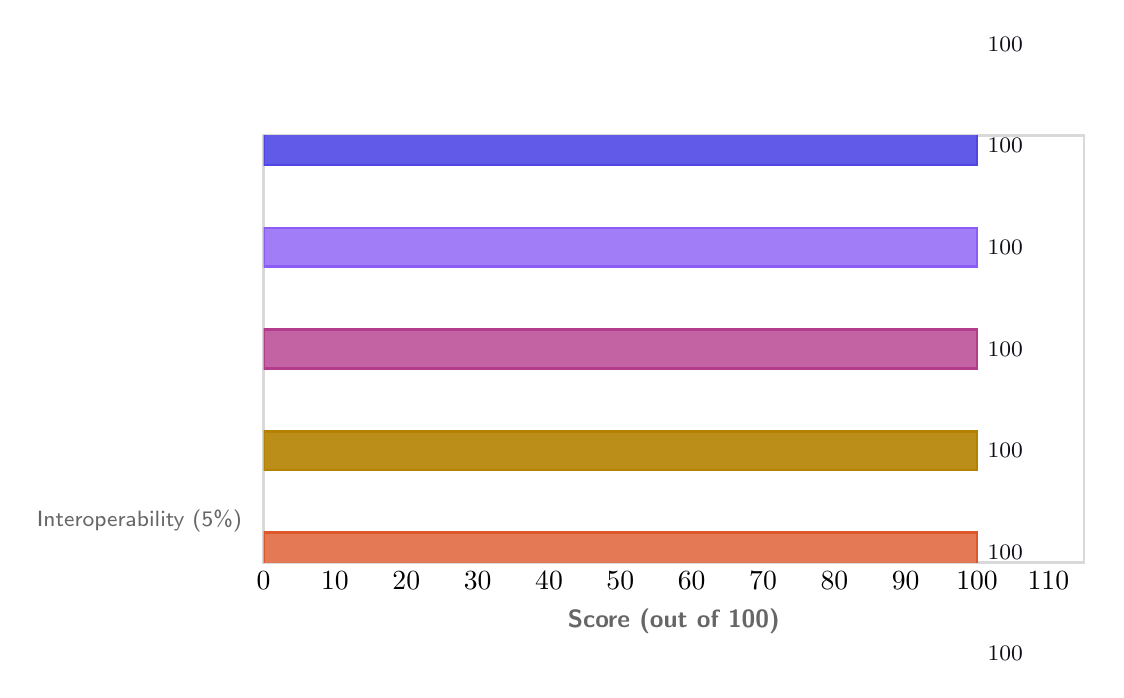
\begin{tikzpicture}
\begin{axis}[
  xbar,
  width=12cm, height=7cm,
  xmin=0, xmax=115,
  xlabel={Score (out of 100)},
  ytick=data,
  yticklabels={
    Interoperability (5\%),
    Armor (10\%),
    Market Fitness (15\%),
    Swarm / A2A (15\%),
    Symbolic Reasoning (15\%),
    Memory (20\%),
    Steel Core (20\%)
  },
  yticklabel style={font=\sffamily\footnotesize, color=gray!80!black},
  nodes near coords,
  nodes near coords align={horizontal},
  every node near coord/.append style={font=\footnotesize\bfseries, color=xdark},
  bar width=14pt,
  enlarge y limits=0.12,
  tick style={draw=none},
  axis line style={draw=gray!30, line width=1pt},
  xlabel style={font=\small\sffamily\bfseries, color=gray!80!black},
  cycle list={
    {fill=xcyan!80,    draw=xcyan, line width=1pt},
    {fill=xrust!80,    draw=xrust, line width=1pt},
    {fill=xgold!90,    draw=xgold, line width=1pt},
    {fill=xpink!80,    draw=xpink, line width=1pt},
    {fill=xamethyst!80,draw=xamethyst, line width=1pt},
    {fill=xblue!90,    draw=xblue, line width=1pt},
    {fill=xblue!70,    draw=xblue!80, line width=1pt}
  }
]
\addplot coordinates { (100,0) };
\addplot coordinates { (100,1) };
\addplot coordinates { (100,2) };
\addplot coordinates { (100,3) };
\addplot coordinates { (100,4) };
\addplot coordinates { (100,5) };
\addplot coordinates { (100,6) };
\end{axis}
\end{tikzpicture}
\caption{ZFI pillar scores (hot Docker mode). All seven pillars achieve 100/100. Each pillar
is rendered in a distinct color corresponding to its architectural layer. Cold-mode (no Docker)
achieves 89.8/100, with the Memory and Swarm pillars partially degraded due to absent
infrastructure services.}
\label{fig:zfi}
\end{figure}

\subsection{Comparison with Existing Systems}

\begin{table}[H]
\centering
\caption{Comparative Analysis (ZFI rubric applied to publicly documented capabilities)}
\resizebox{\textwidth}{!}{%
\begin{tabular}{@{}lcccccc@{}}
\toprule
\textbf{System} & \textbf{ZFI} & \textbf{Local} & \textbf{Symbolic} &
  \textbf{Security} & \textbf{Evolutionary} & \textbf{Multi-Memory}\\
\midrule
\textbf{ZANA (ours)} & \textbf{100.0} & \checkmark & \checkmark & Rust & \checkmark & \checkmark\\
Open Interpreter & $\approx 30$   & \checkmark & $\times$ & $\times$ & $\times$ & $\times$\\
AutoGPT          & $\approx 33$   & $\times$   & $\times$ & $\times$ & $\times$ & $\times$\\
Claude Code      & $\approx 41$   & $\times$   & $\times$ & $\times$ & $\times$ & $\times$\\
N8N + AI         & $\approx 60$   & partial    & $\times$ & partial & $\times$ & $\times$\\
ChatGPT          & $\approx 57$   & $\times$   & $\times$ & cloud   & $\times$ & $\times$\\
\bottomrule
\end{tabular}%
}

\medskip
\noindent\textit{Note: competitor ZFI scores are approximations using ZANA's rubric applied
to publicly documented capabilities; they are not claims by those systems' authors.}
\end{table}

% ===========================================================
\section{Risks, Limitations, and Ethical Considerations}
\label{sec:risks}
% ===========================================================

Deploying a personal cognitive AI at the level of sovereignty that ZANA enables introduces
technical and sociotechnical risks that must be acknowledged explicitly. We structure
these across four dimensions.

\begin{figure}[H]
\centering
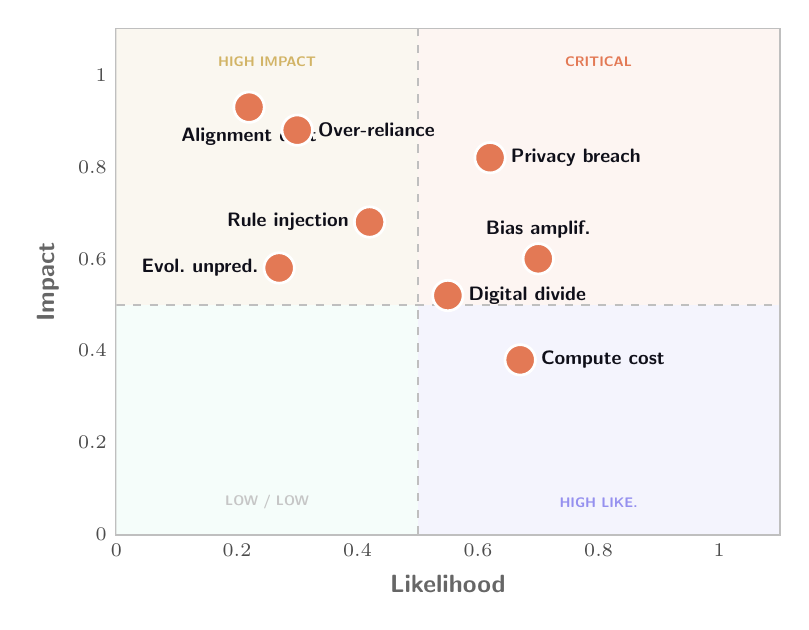
\begin{tikzpicture}
\begin{axis}[
  width=10cm, height=8cm,
  xmin=0, xmax=1.1, ymin=0, ymax=1.1,
  xlabel={Likelihood},
  ylabel={Impact},
  xlabel style={font=\sffamily\small\bfseries, color=gray!80!black},
  ylabel style={font=\sffamily\small\bfseries, color=gray!80!black},
  tick style={draw=gray!40},
  axis line style={draw=gray!50, line width=1pt},
  grid=both,
  grid style={draw=gray!15, line width=0.5pt},
  xticklabel style={font=\sffamily\scriptsize, color=gray!60!black},
  yticklabel style={font=\sffamily\scriptsize, color=gray!60!black},
]
  % Quadrant background fills (placed before data)
  \fill[xrust!6]  (axis cs:0.5,0.5) rectangle (axis cs:1.1,1.1);
  \fill[xgold!6]  (axis cs:0,0.5)   rectangle (axis cs:0.5,1.1);
  \fill[xblue!6]  (axis cs:0.5,0)   rectangle (axis cs:1.1,0.5);
  \fill[xjade!5]  (axis cs:0,0)     rectangle (axis cs:0.5,0.5);
  % Dividing lines
  \draw[gray!50, dashed, line width=0.8pt] (axis cs:0.5,0) -- (axis cs:0.5,1.1);
  \draw[gray!50, dashed, line width=0.8pt] (axis cs:0,0.5) -- (axis cs:1.1,0.5);
  % Quadrant labels (inside axis bounds)
  \node[font=\sffamily\tiny\bfseries, color=gray!45] at (axis cs:0.25,0.07) {LOW / LOW};
  \node[font=\sffamily\tiny\bfseries, color=xblue!60] at (axis cs:0.80,0.07) {HIGH LIKE.};
  \node[font=\sffamily\tiny\bfseries, color=xgold!60] at (axis cs:0.25,1.03) {HIGH IMPACT};
  \node[font=\sffamily\tiny\bfseries, color=xrust!80] at (axis cs:0.80,1.03) {CRITICAL};

  % Risk scatter
  \addplot[only marks,
           mark=*, mark size=5.5pt,
           fill=xrust!80, draw=white, line width=1pt]
    coordinates {
      (0.30, 0.88)   % Over-reliance
      (0.62, 0.82)   % Privacy breach
      (0.22, 0.93)   % Alignment drift
      (0.70, 0.60)   % Bias amplification
      (0.55, 0.52)   % Digital divide
      (0.42, 0.68)   % Rule injection
      (0.27, 0.58)   % Evol. unpredictability
      (0.67, 0.38)   % Compute cost
    };

  % Risk labels — positioned to avoid cluster overlap
  \node[font=\sffamily\scriptsize\bfseries, text=xdark, right, xshift=4pt] at (axis cs:0.30,0.88) {Over-reliance};
  \node[font=\sffamily\scriptsize\bfseries, text=xdark, right, xshift=4pt] at (axis cs:0.62,0.82) {Privacy breach};
  \node[font=\sffamily\scriptsize\bfseries, text=xdark, below, yshift=-4pt] at (axis cs:0.22,0.93) {Alignment drift};
  \node[font=\sffamily\scriptsize\bfseries, text=xdark, above, yshift=4pt]  at (axis cs:0.70,0.60) {Bias amplif.};
  \node[font=\sffamily\scriptsize\bfseries, text=xdark, right, xshift=4pt]  at (axis cs:0.55,0.52) {Digital divide};
  \node[font=\sffamily\scriptsize\bfseries, text=xdark, left,  xshift=-4pt] at (axis cs:0.42,0.68) {Rule injection};
  \node[font=\sffamily\scriptsize\bfseries, text=xdark, left,  xshift=-4pt] at (axis cs:0.27,0.58) {Evol.\ unpred.};
  \node[font=\sffamily\scriptsize\bfseries, text=xdark, right, xshift=4pt]  at (axis cs:0.67,0.38) {Compute cost};
\end{axis}
\end{tikzpicture}
\caption{Risk landscape for sovereign personal AI systems. Risks are plotted by estimated
likelihood (horizontal axis) and potential impact (vertical axis). High-impact, high-likelihood
risks (upper-right quadrant) receive priority attention in Sections~\ref{sec:risks:tech}
and~\ref{sec:risks:socio}.}
\label{fig:risks}
\end{figure}

\subsection{Technical Risks}
\label{sec:risks:tech}

\begin{tcolorbox}[riskbox, title={Risk T1: Alignment Drift in Evolved Warriors}]
\textbf{Description:} Idle Zero evolves warrior algorithms over 2000 generations using fitness
functions defined on personal data. Over time, if the personal data itself contains biases,
the evolved warriors may amplify those biases.\\
\textbf{Likelihood:} Low (requires adversarial data + extended evolution).\\
\textbf{Mitigation:} LLMGuard validates warrior genomes before promotion to procedural memory.
Civic Ledger (Milestone 8.1) provides an auditable history of every promoted champion.
\end{tcolorbox}

\begin{tcolorbox}[riskbox, title={Risk T2: Rule Injection via Swarm Synchronization}]
\textbf{Description:} Milestone 8.3 introduces remote rule synchronization from swarm peers.
A malicious peer could inject a logical rule designed to alter the system's behavior
(e.g., ``IF query contains keyword $k$ THEN assert false fact $f$'').\\
\textbf{Likelihood:} Medium (requires malicious peer in swarm).\\
\textbf{Mitigation:} \texttt{LLMGuard} scans all incoming rules. Cryptographic signatures
(SHA-256 Civic Ledger) make rule provenance auditable and traceable.
\end{tcolorbox}

\begin{tcolorbox}[riskbox, title={Risk T3: Evolutionary Unpredictability}]
\textbf{Description:} The Red Queen tournament, by design, evolves towards adversarial
novelty. A champion warrior may discover a strategy that is high-fitness on the training
distribution but exhibits unpredictable behavior on out-of-distribution inputs.\\
\textbf{Likelihood:} Low-Medium.\\
\textbf{Mitigation:} Champions are quarantined in \texttt{champions/} and require explicit
promotion by the operator. The symbolic engine verifies all warrior outputs before they
can assert facts.
\end{tcolorbox}

\subsection{Sociotechnical Risks}
\label{sec:risks:socio}

\begin{tcolorbox}[riskbox, title={Risk S1: Epistemic Over-Reliance}]
\textbf{Description:} An operator who delegates all decision-making to ZANA may atrophy
the cognitive skills that ZANA augments. This mirrors concerns about GPS navigation
and spatial reasoning.\\
\textbf{Likelihood:} High (common pattern with any powerful tool).\\
\textbf{Mitigation:} ZANA is designed as a \emph{co-pilot}, not an autonomous agent.
The Apex Quintet always surfaces its reasoning trace; the operator is expected to
review, not simply accept.
\end{tcolorbox}

\begin{tcolorbox}[riskbox, title={Risk S2: Privacy Breach via Episodic Leakage}]
\textbf{Description:} ZANA's episodic store accumulates a high-resolution record of
the operator's cognition over years. If this store is compromised (device theft,
software vulnerability), the exposure is far more intimate than conventional data leaks.\\
\textbf{Likelihood:} High (any local-first system with persistent storage faces this).\\
\textbf{Mitigation:} AES-256-GCM encryption with hardware binding. The Armor layer
prevents exfiltration via the LLM. Users are strongly advised to encrypt the storage
volume at the OS level.
\end{tcolorbox}

\begin{tcolorbox}[riskbox, title={Risk S3: Digital Divide Amplification}]
\textbf{Description:} ZANA's full stack (Docker + GPU for local LLM + Rust compilation)
requires hardware inaccessible to much of the global population. An effective cognitive
augmentation tool available only to the already-privileged amplifies existing inequalities.\\
\textbf{Likelihood:} High (structural, not contingent).\\
\textbf{Mitigation:} The cold-mode path (ZFI = 89.8, no Docker required) runs on
consumer hardware. Groq/OpenRouter fallback enables cloud LLMs for operators without
local GPU. Long-term: lightweight Rust binary target for sub-\$100 single-board computers.
\end{tcolorbox}

\begin{tcolorbox}[riskbox, title={Risk S4: Dual-Use for Surveillance}]
\textbf{Description:} ZANA's multimodal sensing (audio via Whisper, vision via LLaVA)
combined with continuous episodic logging could be repurposed for surveillance of
third parties without consent.\\
\textbf{Likelihood:} Medium.\\
\textbf{Mitigation:} The MIT License does not restrict use, but the architecture includes
explicit PII protections. We call on deployers to adhere to applicable privacy law
(GDPR, CCPA). Future work includes a consent framework integrated at the sensor layer.
\end{tcolorbox}

\subsection{Ethical Principles for Deployment}

We propose four non-negotiable principles for responsible ZANA deployment:

\begin{enumerate}[leftmargin=*, label=\textbf{P\arabic*.}]
  \item \textbf{Operator Transparency:} ZANA must surface its reasoning trace on request.
    No ``black box'' decisions. The Civic Ledger is the mechanism.
  \item \textbf{Consent Boundaries:} Multimodal sensing must be enabled explicitly for each
    input channel. No ambient recording without operator consent.
  \item \textbf{Right to Delete:} The operator must be able to purge any memory store at
    any time. ZANA owns no data; the operator owns everything.
  \item \textbf{Interoperability Obligation:} ZANA's data formats (AION protocol, DNA files)
    must remain open and documented so operators can migrate away at will.
\end{enumerate}

% ===========================================================
\section{Discussion}
% ===========================================================

\subsection{Architectural Insights}

The seven-layer stack reflects a key design philosophy: \emph{verification before enrichment,
enrichment before inference, inference before action}. Each layer can fail independently ---
Armor rejects malicious inputs before the Kalman filter sees them, and the symbolic engine
can reject LLM outputs before the Apex Quintet acts on them. This independence is what makes
ZANA's security model structural rather than probabilistic.

The EML operator's role deserves particular emphasis. By reducing all arithmetic to a single
primitive, ZANA achieves a level of mathematical auditability that complex floating-point
pipelines cannot. In a world where AI systems make consequential decisions in finance,
healthcare, and law, reproducibility is not a convenience --- it is an ethical requirement.

\subsection{The Sovereignty Principle in Context}

ZANA's ``zero'' in its name (Zero Autonomous Neural Architecture) reflects an important
inversion: most AI products maximize the AI's autonomy at the expense of the operator's
sovereignty. ZANA inverts this. The system executes with maximum capability while keeping
every decision transparent, every memory accessible, and every computation reproducible.

This is not a technical constraint but a design axiom. Future AI architectures that aspire
to genuine usefulness for individuals --- not just enterprises --- must take this inversion
seriously.

\subsection{Limitations}

\textbf{Rust compilation complexity.} Steel Core and Armor require Rust 1.78+ with AVX2.
Users on ARM or non-AVX2 x86 must remove \texttt{-C target-cpu=native} from the build flags.

\textbf{Foundation model dependency.} Best reasoning quality requires a capable LLM (Claude
Sonnet or equivalent). The symbolic layer compensates substantially but cannot fully substitute
on resource-constrained hardware.

\textbf{Single-node deployment.} Distributed swarm reasoning (Milestone~8.3) is designed
but not yet implemented.

\textbf{Red Queen convergence time.} The 2000-generation tournament is CPU-intensive.
\texttt{rayon} parallelism mitigates this, but it remains unsuitable for embedded devices.

\textbf{Benchmark self-reference.} The ZFI benchmark was designed by the same team that
built ZANA. While we have made every effort to make the rubric objective and publicly
documented, independent external evaluation is a critical next step.

\subsection{Future Work}
\label{sec:future}

\textbf{Milestone 8.1 --- Civic Ledger.} Mirror the rule base to a SHA-256 audit log,
making every rule change publicly auditable through the UI.

\textbf{Milestone 8.2 --- Mastery Map.} Link rule assimilation to operator progression
metrics, enabling a measurable ``cognitive fitness'' trajectory.

\textbf{Milestone 8.3 --- Remote Swarm Query.} Broadcast \texttt{RemoteQuery} to peer
nodes when the local engine has no applicable rule. Peer responses are scored by LLMGuard
before loading.

\textbf{Online Red Queen.} Integrate the tournament loop with live interaction data,
combining curriculum learning~\cite{bengio2009curriculum} with real-time feedback.

\textbf{LLM personalization via model merging.} Following~\cite{akiba2024modelmerging},
champion warrior algorithms could guide low-rank adaptations of the local LLM weights,
producing a personalized model without full fine-tuning.

\textbf{Independent ZFI validation.} Publish the ZFI benchmark suite as a standalone
repository so that any system can be evaluated against the same rubric by an independent
party.

% ===========================================================
\section{Conclusion}
% ===========================================================

ZANA demonstrates that a personal cognitive AI can simultaneously satisfy epistemic rigor,
security guarantees, emotional awareness, evolutionary self-improvement, and practical
deployability --- without sacrificing operator sovereignty.

We have made the following contributions:

\begin{enumerate}[leftmargin=*, label=\arabic*.]
  \item A \textbf{formal cognitive state-space theory} grounding the Kalman filter,
    information-theoretic context management, neuro-symbolic integration, EML completeness,
    and fuzzy emotional modulation in established mathematical frameworks.
  \item A \textbf{seven-layer neuro-symbolic architecture} where each layer adds
    verification or enrichment before passing the payload to the next.
  \item \textbf{Security-by-architecture}: Rust Armor makes PII and injection checks
    impossible to bypass through the Python application layer, at $2.1\,\mu$s per call.
  \item A \textbf{Digital Red Queen tournament} (Idle Zero) that adversarially evolves
    typed cognitive algorithms and crystallizes champions back into the procedural
    memory registry.
  \item A \textbf{typed inter-agent protocol} (AION) that eliminates hallucination cascade
    in five-agent Apex Quintet pipelines.
  \item A \textbf{reproducible seven-pillar benchmark} (ZFI) with a reference implementation
    achieving $100.0/100$ on a standard workstation.
  \item A \textbf{taxonomy of eight application domains} with three detailed case studies.
  \item A \textbf{structured risk analysis} covering eight technical and sociotechnical risks
    with concrete mitigations.
\end{enumerate}

ZANA is released in full --- Rust, Python, TypeScript, Docker compose, benchmark suite ---
under the MIT License at \url{https://github.com/kemquiros/zana-core}. The goal is not to
build a product but to establish a reference architecture: a proof that personal cognitive AI
can be rigorous, sovereign, and open.

\bigskip
\begin{center}
{\large\itshape Este es mi regalo para el mundo.}
\end{center}

% ===========================================================
\section*{Acknowledgements}
% ===========================================================

The author thanks the open-source communities behind Rust, PyO3, FastAPI, ChromaDB, Neo4j,
LangGraph, smolagents, and Ollama. Special recognition to Lotfi A.\ Zadeh for the mathematical
foundations of approximate reasoning; Rudolf E.\ Kalman for the optimal estimation framework
that underpins the Steel Core; David Ha and J\"{u}rgen Schmidhuber for the world-model framing;
the team at Sakana AI for the Digital Red Queen paper that inspired the Idle Zero tournament;
and Andrej Karpathy for articulating the engineering discipline that shaped this architecture's
design principles.

% ===========================================================
\bibliographystyle{plain}
\begin{thebibliography}{99}

\bibitem{kalman1960filter}
R.~E. Kalman.
\newblock A new approach to linear filtering and prediction problems.
\newblock \emph{Journal of Basic Engineering}, 82(1):35--45, 1960.

\bibitem{tulving1985elements}
E.~Tulving.
\newblock \emph{Elements of Episodic Memory}.
\newblock Oxford University Press, 1983.

\bibitem{zadeh1965fuzzysets}
L.~A. Zadeh.
\newblock Fuzzy sets.
\newblock \emph{Information and Control}, 8(3):338--353, 1965.

\bibitem{zadeh1973outline}
L.~A. Zadeh.
\newblock Outline of a new approach to the analysis of complex systems and
  decision processes.
\newblock \emph{IEEE Transactions on Systems, Man, and Cybernetics},
  3(1):28--44, 1973.

\bibitem{zadeh1975fuzzylogic}
L.~A. Zadeh.
\newblock Fuzzy logic and approximate reasoning.
\newblock \emph{Synthese}, 30(3--4):407--428, 1975.

\bibitem{mamdani1974application}
E.~H. Mamdani.
\newblock Application of fuzzy algorithms for control of simple dynamic plant.
\newblock \emph{Proceedings of the Institution of Electrical Engineers},
  121(12):1585--1588, 1974.

\bibitem{takagi1985fuzzy}
T.~Takagi and M.~Sugeno.
\newblock Fuzzy identification of systems and its applications to modeling and
  control.
\newblock \emph{IEEE Transactions on Systems, Man, and Cybernetics},
  15(1):116--132, 1985.

\bibitem{ha2018worldmodels}
D.~Ha and J.~Schmidhuber.
\newblock World models.
\newblock \emph{arXiv preprint arXiv:1803.10122}, 2018.

\bibitem{ng2000irl}
A.~Y. Ng and S.~J. Russell.
\newblock Algorithms for inverse reinforcement learning.
\newblock In \emph{Proc.\ 17th ICML}, pages 663--670, 2000.

\bibitem{bengio2009curriculum}
Y.~Bengio, J.~Louradour, R.~Collobert, and J.~Weston.
\newblock Curriculum learning.
\newblock In \emph{Proc.\ 26th ICML}, pages 41--48, 2009.

\bibitem{real2020automlzero}
E.~Real, C.~Liang, D.~R. So, and Q.~V. Le.
\newblock {AutoML-Zero}: Evolving machine learning algorithms from scratch.
\newblock In \emph{Proc.\ 37th ICML}, 2020.

\bibitem{kumar2025redqueen}
A.~Kumar, R.~Bahlous-Boldi, P.~Sharma, P.~Isola, S.~Risi, Y.~Tang,
  and D.~Ha.
\newblock Digital red queen: Adversarial program evolution in {C}ore {W}ar
  with {LLM}s.
\newblock \emph{arXiv:2601.03335}, 2025.

\bibitem{akiba2024modelmerging}
T.~Akiba, M.~Shing, Y.~Tang, Q.~Sun, and D.~Ha.
\newblock Evolutionary optimization of model merging recipes.
\newblock \emph{Nature Machine Intelligence}, 2025.

\bibitem{lu2024preferenceoptalgo}
C.~Lu et~al.
\newblock Discovering preference optimization algorithms with and for large
  language models.
\newblock In \emph{NeurIPS}, 2024.

\bibitem{bates1994emotion}
J.~Bates.
\newblock The role of emotion in believable agents.
\newblock \emph{Communications of the ACM}, 37(7):122--125, 1994.

\bibitem{odrzywolekEML}
A.~Odrzyw{o\l}ek.
\newblock All elementary functions from a single binary operator.
\newblock \emph{arXiv:2603.21852}, 2026.

\bibitem{anderson2004actr}
J.~R. Anderson et~al.
\newblock An integrated theory of the mind.
\newblock \emph{Psychological Review}, 111(4):1036--1060, 2004.

\bibitem{laird2012soar}
J.~E. Laird.
\newblock \emph{The {S}oar Cognitive Architecture}.
\newblock MIT Press, 2012.

\bibitem{greshake2023promptinjection}
K.~Greshake et~al.
\newblock Not what you've signed up for: Compromising real-world
  {LLM}-integrated applications with indirect prompt injection.
\newblock In \emph{AISec Workshop, ACM CCS}, 2023.

\bibitem{langchain2024langgraph}
LangChain.
\newblock {LangGraph}: Building stateful, multi-actor {LLM} applications, 2024.
\newblock \url{https://github.com/langchain-ai/langgraph}.

\bibitem{huggingface2024smolagents}
HuggingFace.
\newblock smolagents: A minimal framework for agentic {AI}, 2024.
\newblock \url{https://github.com/huggingface/smolagents}.

\bibitem{knuth1997art}
D.~E. Knuth.
\newblock \emph{The Art of Computer Programming, Vol.\ 1: Fundamental
  Algorithms}, 3rd ed.
\newblock Addison-Wesley, 1997.

\bibitem{cohen1980preserved}
N.~J. Cohen and L.~R. Squire.
\newblock Preserved learning and retention of pattern-analyzing skill in
  amnesia: Dissociation of knowing how and knowing that.
\newblock \emph{Science}, 210(4466):207--210, 1980.

\bibitem{vecanova2026}
VECANOVA.
\newblock {KoruOS}: The Operating System of the Self --- system architecture
  and product vision, 2026.
\newblock Internal technical document. \url{https://vecanova.com}.

\end{thebibliography}

% ===========================================================
\newpage
\section*{Glossary}
% ===========================================================

\begin{description}[leftmargin=3cm, style=nextline, font=\bfseries\color{xblue}]

  \item[ZANA]
    \emph{Zero Autonomous Neural Architecture.} The cognitive AI runtime presented
    in this paper. A seven-layer neuro-symbolic system designed for sovereign,
    local-first personal cognitive augmentation.

  \item[KoruOS]
    \emph{Operating System of the Self.} VECANOVA's flagship product ecosystem.
    ZANA is the cognitive engine at its core. KoruOS encompasses the full stack:
    ARIA UI, ZANA Core, and the distributed Swarm infrastructure.

  \item[VECANOVA]
    AI solutions company and parent entity of the KoruOS ecosystem. Develops
    sovereign AI products for individuals and organizations.

  \item[ZFI]
    \emph{ZANA Fitness Index.} A seven-pillar composite benchmark (Steel Core,
    Memory, Symbolic Reasoning, Swarm/A2A, Market Fitness, Armor,
    Interoperability) scored 0--100. Reference implementation achieves 100.0/100.

  \item[AION]
    \emph{Artificial Intelligence Ontological Notation.} The typed inter-agent
    communication protocol used by the Apex Quintet. Messages carry latent state
    vectors, Bayesian innovation signals, EML trees, and IRL reward expectations.
    Plain-text fields are structurally absent.

  \item[EML]
    \emph{Exponential-Log operator.} A universal arithmetic primitive
    $\mathrm{eml}(x,y) = e^x - \ln y$ from which all elementary functions can be
    derived. Used in the Steel Core for arithmetic determinism.

  \item[Aeon]
    A specialized ZANA instance with its own evolutionary DNA (SDA file).
    Aeons can be adopted, traded, or promoted within the swarm. Evolution
    stages: Seed → Larva → Warrior → Aeon → Singularity.

  \item[SDA / DNA]
    \emph{Self-Describing Architecture.} A serializable file encoding an Aeon's
    architecture, weights, and thresholds. Enables portable cognitive genomes.

  \item[Shadow Observer]
    A Rust-native daemon ($<$10 MB RAM) that captures passive context (window
    focus, document titles, clipboard) as implicit operator signals. Feeds the
    Fuzzy Heart's surprise computation.

  \item[Steel Core]
    The Rust-native high-performance computation layer. Contains the Cognitive
    Kalman Filter, EML operator, and Policy Brain. Accessed via PyO3 zero-copy
    buffers at $<$10\,$\mu$s latency.

  \item[Armor]
    Rust middleware for structural security. Inspects every input and output
    for PII and prompt-injection patterns at $2.1\,\mu$s per call.
    Cannot be bypassed through the Python application layer.

  \item[IRL Engine]
    \emph{Inverse Reinforcement Learning Engine.} Recovers the operator's latent
    reward function from implicit correction signals (accept/edit/reject).
    Updates procedural Q-values without explicit reward specification.

  \item[Curriculum Manager]
    Manages the skill DAG --- a Directed Acyclic Graph of 54 base modules
    ordered by prerequisite dependency. Focuses Red Queen evolutionary pressure
    on the skill branch identified by the IRL Engine.

  \item[Apex Quintet]
    The five specialized agents forming ZANA's orchestration layer:
    \textbf{Sentinel} (security), \textbf{Archivist} (retrieval),
    \textbf{Analyst} (reasoning), \textbf{Operator} (execution),
    \textbf{Herald} (synthesis). They communicate exclusively via AION.

  \item[Fuzzy Heart]
    The emotional modulation subsystem. Maps affect-space inputs
    (surprise, valence, arousal) to a mood vector via Mamdani fuzzy inference,
    adjusting LLM sampling temperature accordingly.

  \item[Red Queen Tournament]
    Adversarial evolutionary loop in Idle Zero. Fifty warrior algorithms
    compete over 2000 generations. Champions are crystallized and promoted
    to the procedural memory registry.

\end{description}

\end{document}
